\documentclass[twocolumn,english]{article}
\usepackage[latin9]{inputenc}
\usepackage[landscape]{geometry}
\geometry{verbose,tmargin=0.5in,bmargin=0.75in,lmargin=0.5in,rmargin=0.5in}
\setlength{\parskip}{0bp}
\setlength{\parindent}{0pt}
\usepackage{array}
\usepackage{float}
\usepackage{booktabs}
\usepackage{multirow}
\usepackage{amstext}
\usepackage{graphicx}

\makeatletter

\providecommand{\tabularnewline}{\\}

\setlength{\columnsep}{0.25in}
\usepackage{xcolor}
\usepackage{textcomp}
\usepackage{listings}
\lstset{
  language=haskell,
  tabsize=2,
  basicstyle=\small\ttfamily,
}

\@ifundefined{showcaptionsetup}{}{%
 \PassOptionsToPackage{caption=false}{subfig}}
\usepackage{subfig}
\makeatother

\usepackage{babel}
\begin{document}

\title{Reference Sheet for C112 Hardware}


\date{Autumn 2016}

\maketitle

\section{Boolean Algebra, Gates and Circuits}


\paragraph{Basic Operators}

Precedence : (strongest) $'$, $\cdot$, $+$ (weakest).

\begin{table}[H]
\noindent \centering{}%
\begin{tabular}{ccc}
\toprule 
\multicolumn{3}{c}{AND $\cdot$}\tabularnewline
A & B & \textbf{R}\tabularnewline
\midrule
0 & 0 & \textbf{0}\tabularnewline
0 & 1 & \textbf{0}\tabularnewline
1 & 0 & \textbf{0}\tabularnewline
1 & 1 & \textbf{1}\tabularnewline
\bottomrule
\end{tabular} %
\begin{tabular}{ccc}
\toprule 
\multicolumn{3}{c}{OR $+$}\tabularnewline
A & B & \textbf{R}\tabularnewline
\midrule
0 & 0 & \textbf{0}\tabularnewline
0 & 1 & \textbf{1}\tabularnewline
1 & 0 & \textbf{1}\tabularnewline
1 & 1 & \textbf{1}\tabularnewline
\bottomrule
\end{tabular} %
\begin{tabular}{cc}
\toprule 
\multicolumn{2}{c}{NOT $'$}\tabularnewline
A & \textbf{R}\tabularnewline
\midrule
0 & \textbf{1}\tabularnewline
1 & \textbf{0}\tabularnewline
\bottomrule
\end{tabular}
\end{table}



\paragraph{Simplification Rules}
\begin{itemize}
\item AND and OR are associative, commutative and distributive.
\item $\left(A'\right)'=A$.
\item $A\cdot A'=0$ and $A+A'=1$.
\item $A\cdot A=A$ and $A+A=A$.
\item $A\cdot0=0$ and $A+1=1$.
\item $A\cdot1=A$ and $A+0=A$.
\item $\left(A+B\right)'=A'\cdot B'$ and $\left(A\cdot B\right)'=A'+B'$
(De Morgan's).
\end{itemize}
Note that:
\begin{itemize}
\item Each equation has a dual (swap AND with OR and 0 with 1).
\item De Morgan's holds for any number of terms.
\end{itemize}
\textbf{Gates}

There are 4 possible one-input and 16 possible two-input gates. NAND
and NOR are preferred (small and fast).

\begin{figure}[H]
\noindent \begin{centering}
\subfloat{\noindent \centering{}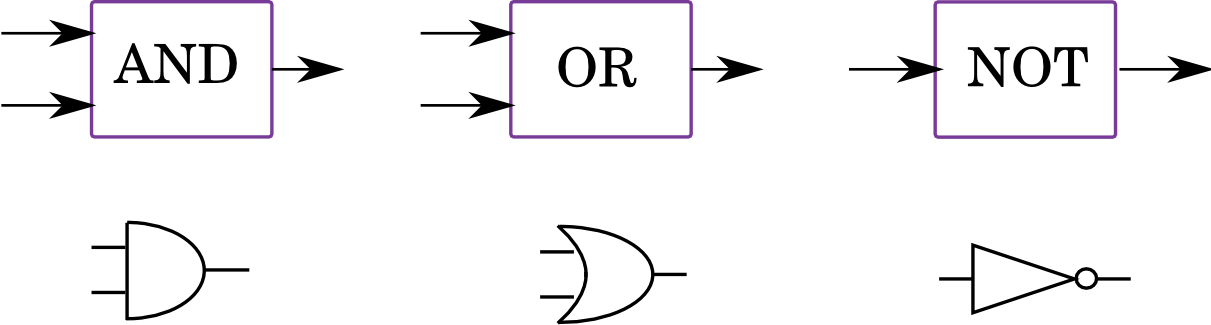
\includegraphics[width=0.25\paperwidth]{img/and}}
\par\end{centering}

\bigskip{}


\noindent \begin{centering}
\subfloat{\noindent \centering{}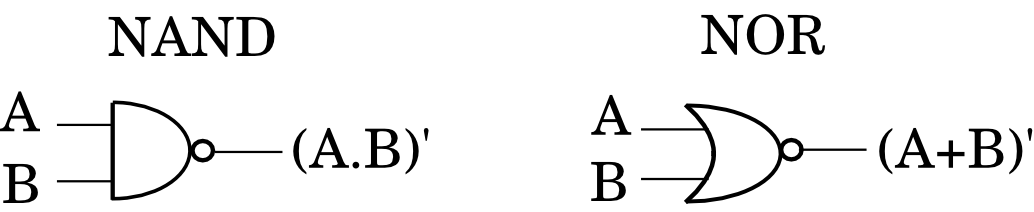
\includegraphics[width=0.25\textwidth]{img/nand}}
\par\end{centering}

\bigskip{}


\noindent \centering{}\subfloat{\noindent \centering{}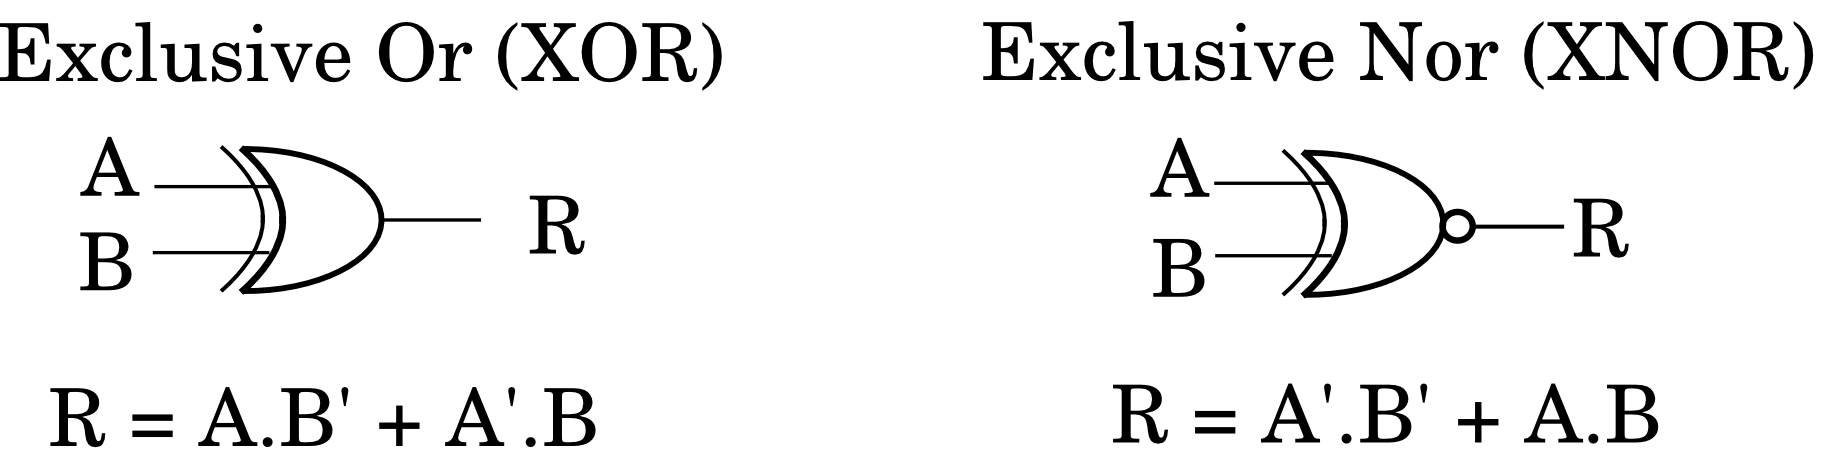
\includegraphics[width=0.25\paperwidth]{img/xor}}
\end{figure}



\paragraph{Analysing Circuits}

Work systematically, building up a formula or truth table in stages.


\paragraph{Simplifying Circuits}

Use De Morgan's:

\begin{figure}[H]
\noindent \centering{}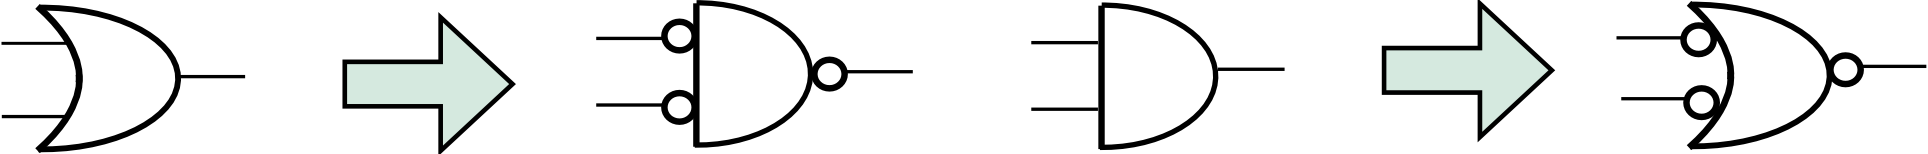
\includegraphics[width=0.25\paperwidth]{img/simplify}
\end{figure}



\paragraph{Control and Data Variables}

E.g. in a multiplexer:

\begin{figure}[H]
\noindent \centering{}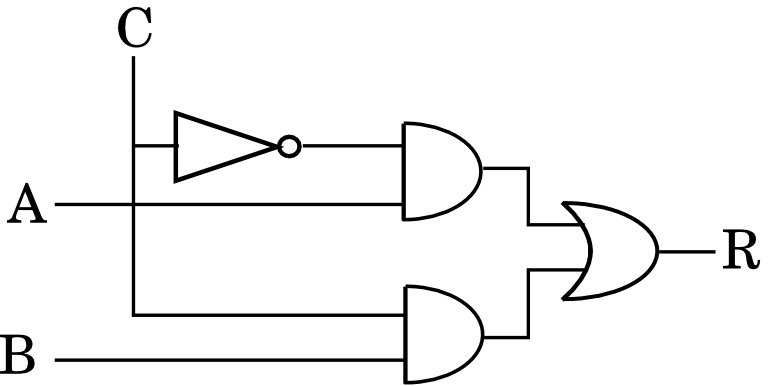
\includegraphics[width=0.15\paperwidth]{img/mux}
\end{figure}



\section{Combinatorial Circuits}


\paragraph{Minterms and Maxterms}
\begin{itemize}
\item \emph{Minterm}: Boolean product term in which for each input, $A_{k}$,
$A_{k}$ or $A_{k}'$ appears exactly once.
\item \emph{Maxterm}: Boolean sum term ....
\end{itemize}

\paragraph{Cannonical Forms}
\begin{itemize}
\item \emph{Minterm Cannonical Form}: Boolean sum of all minterms that ouput
1.
\item \emph{Maxterm Cannonical Form}: Boolean product of all maxterms that
output 0.
\end{itemize}

\paragraph{Karnaugh Maps}

E.g.

\begin{figure}[H]
\noindent \centering{}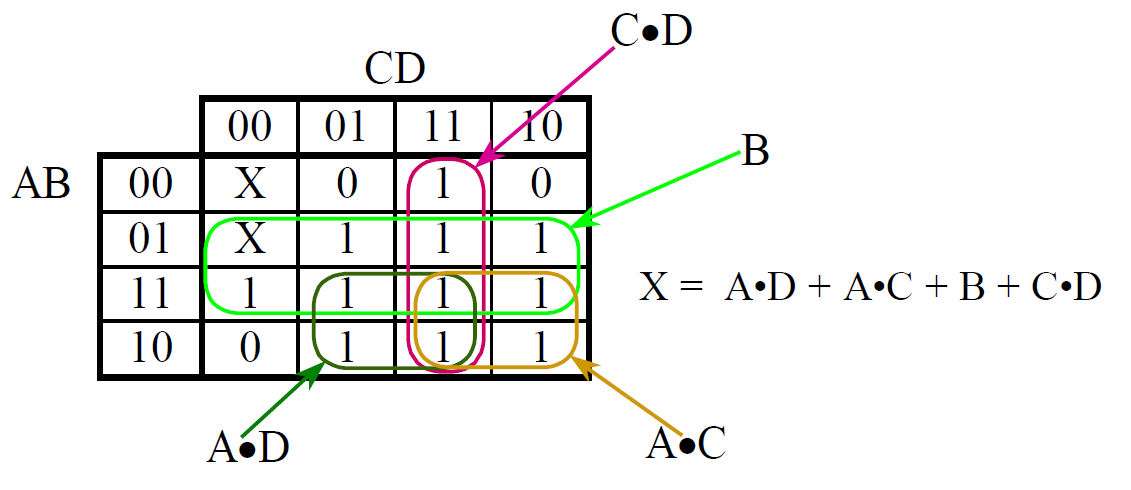
\includegraphics[width=0.25\paperwidth]{img/kmap}
\end{figure}


Remember:
\begin{itemize}
\item \emph{Order} (00, 01, 11, 10) is important.
\item K-maps are \emph{cyclic}.
\item We might be able to make a considerable simplification by considering
\emph{maxterms} (0s) instead of minterms.
\item \emph{Don't cares} (X) can be 0 or 1 - value depends on whether not
they are circled.
\end{itemize}

\paragraph{Combinatorial Circuit \emph{Design Process}}
\begin{enumerate}
\item Generate the truth table.
\item Generate the Karnaugh map.
\item Find the minimal Boolean Expression:

\begin{enumerate}
\item Read off the K-map.
\item Factor out any common factors.
\end{enumerate}
\item Draw the circuit.
\item Minimise to suit production method:

\begin{enumerate}
\item Reduce size (e.g. replace OR, AND by NAND, NOR).
\item Improve speed (reduce cycles).
\end{enumerate}
\item Test the circuit (e.g. systematic testing, formal verificaiton).
\end{enumerate}

\section{Physical Implementation}


\paragraph{Models of the Transistor}

Need to take into account a time delay.

\begin{table}[H]
\noindent \begin{minipage}[t]{0.1\textwidth}

\subfloat{\noindent \centering{}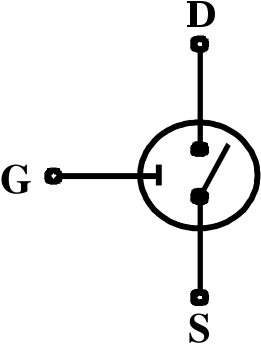
\includegraphics[width=0.08\paperwidth]{img/transistor-simple} }

\noindent \end{minipage}
\begin{minipage}[c]{0.4\textwidth}
\begin{enumerate}
\item \noindent \emph{Procedural model}:

\begin{enumerate}
\item $G,D$and $G,S$ not connected.
\item If $V_{GS}<0.5$V: switch open.
\item If $V_{GS}>1.7$V: switch closed.
\end{enumerate}
\item \emph{Time Delay}:

\begin{enumerate}
\item It takes a constant time for the transistor to which states - can
lead to spikes.
\end{enumerate}
\item \emph{Change is not Instantaneous}:

\begin{enumerate}
\item Account for capacitance: $I=C\frac{\mbox{d}V}{\mbox{d}t}$.
\end{enumerate}
\end{enumerate}
\noindent \centering{}\end{minipage}
\end{table}


Ideal change is 0 - 5V, but actually is somewhere close 0.2 - 3.7V
(with 0.5 - 1.7V considered non-deterministic).

\begin{figure}[H]
\noindent \centering{}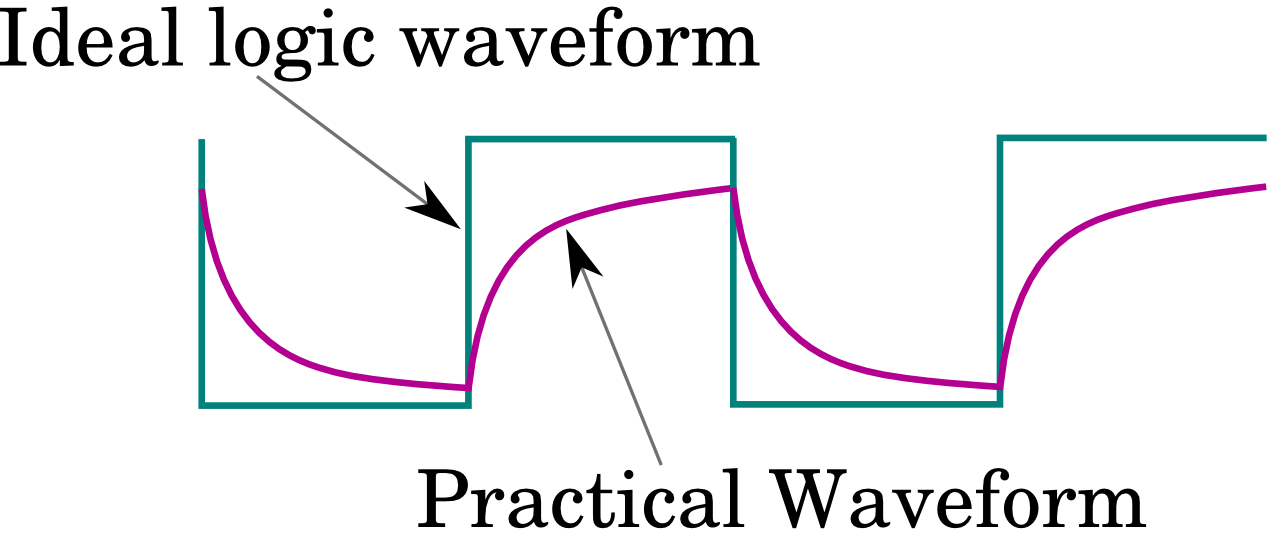
\includegraphics[width=0.15\paperwidth]{img/waveform}
\end{figure}


\begin{figure}[H]
\textbf{Basic Gate Implementations}

\noindent \begin{centering}
NOT
\par\end{centering}

\noindent \begin{centering}
\subfloat{\noindent \centering{}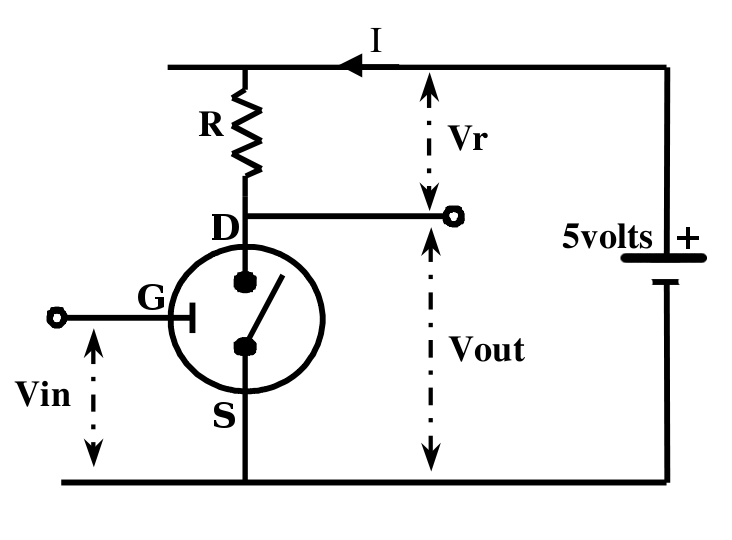
\includegraphics[width=0.2\paperwidth]{img/notgate}}
\par\end{centering}

\noindent \begin{centering}
NAND and NOR
\par\end{centering}

\noindent \centering{}\subfloat{\noindent \centering{}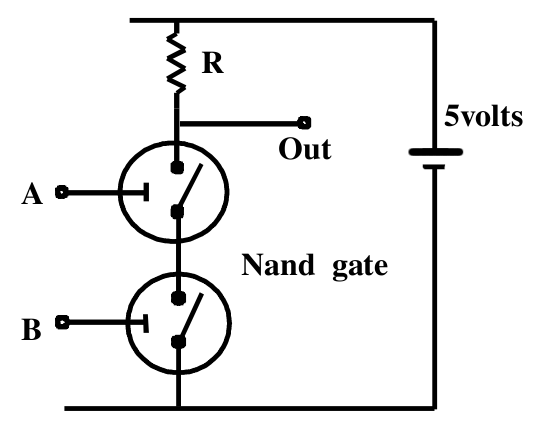
\includegraphics[width=0.15\textwidth]{img/nandgate}}\subfloat{\noindent \centering{}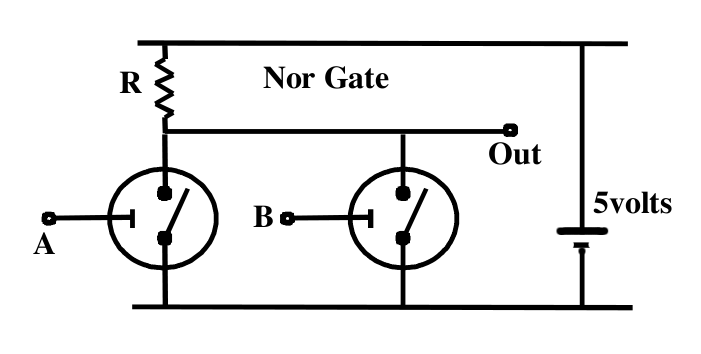
\includegraphics[width=0.175\paperwidth]{img/norgate}}
\end{figure}


Actual ICs generally use a combination of NMOS and PMOS (\textbf{C}omplimentary
\textbf{M}etal \textbf{O}xide \textbf{S}ilicon) instead of resistors
- lower power consumption and faster switching.

\begin{figure}[H]
\textbf{Time Dependent Behaviour of Circuits}

\noindent \centering{}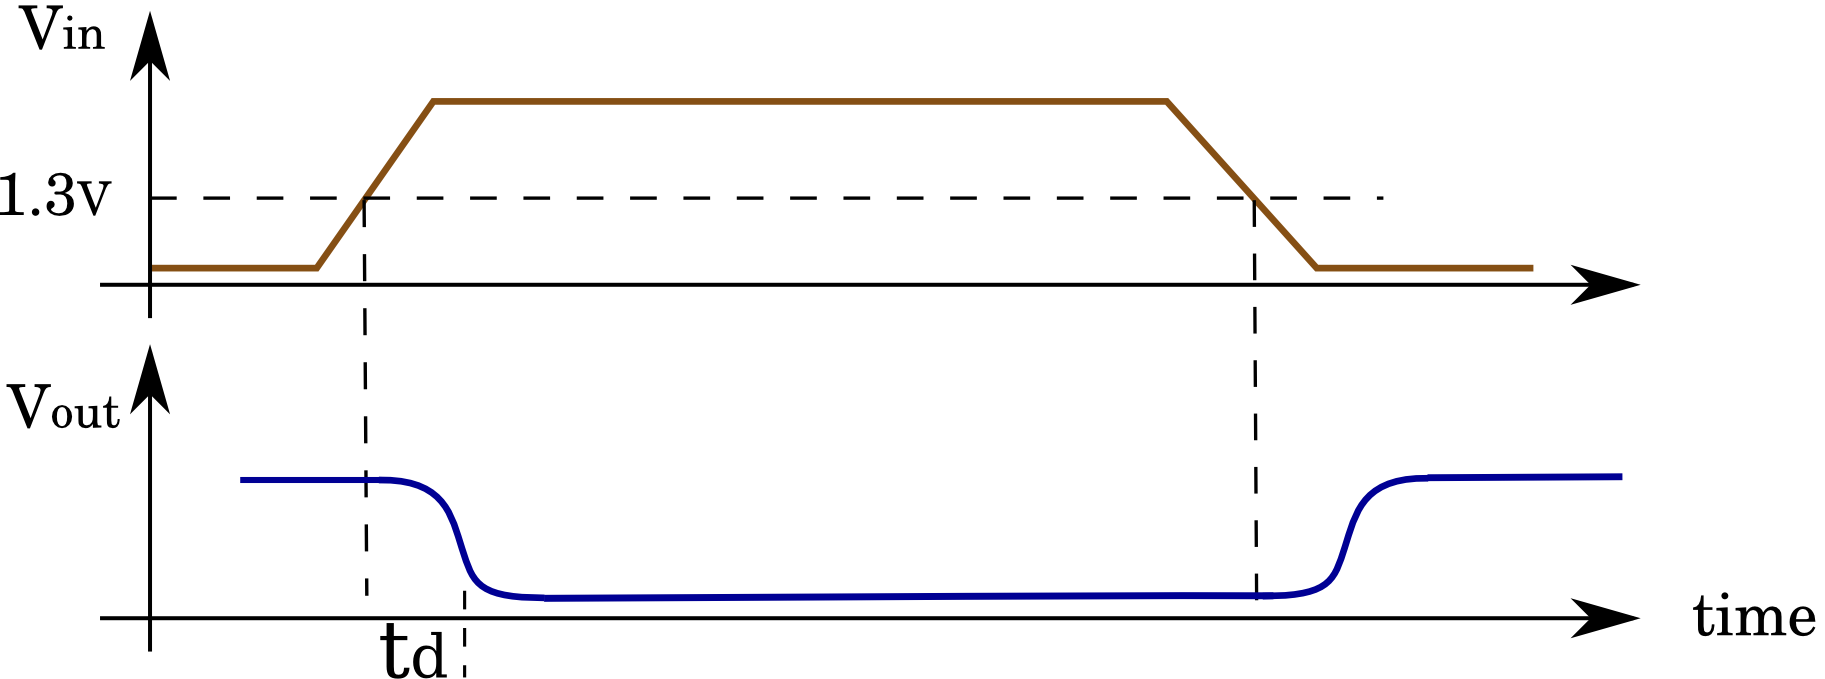
\includegraphics[width=0.25\paperwidth]{img/td}
\end{figure}


\begin{figure}[H]
\noindent \textbf{Noise Margin}

\noindent \centering{}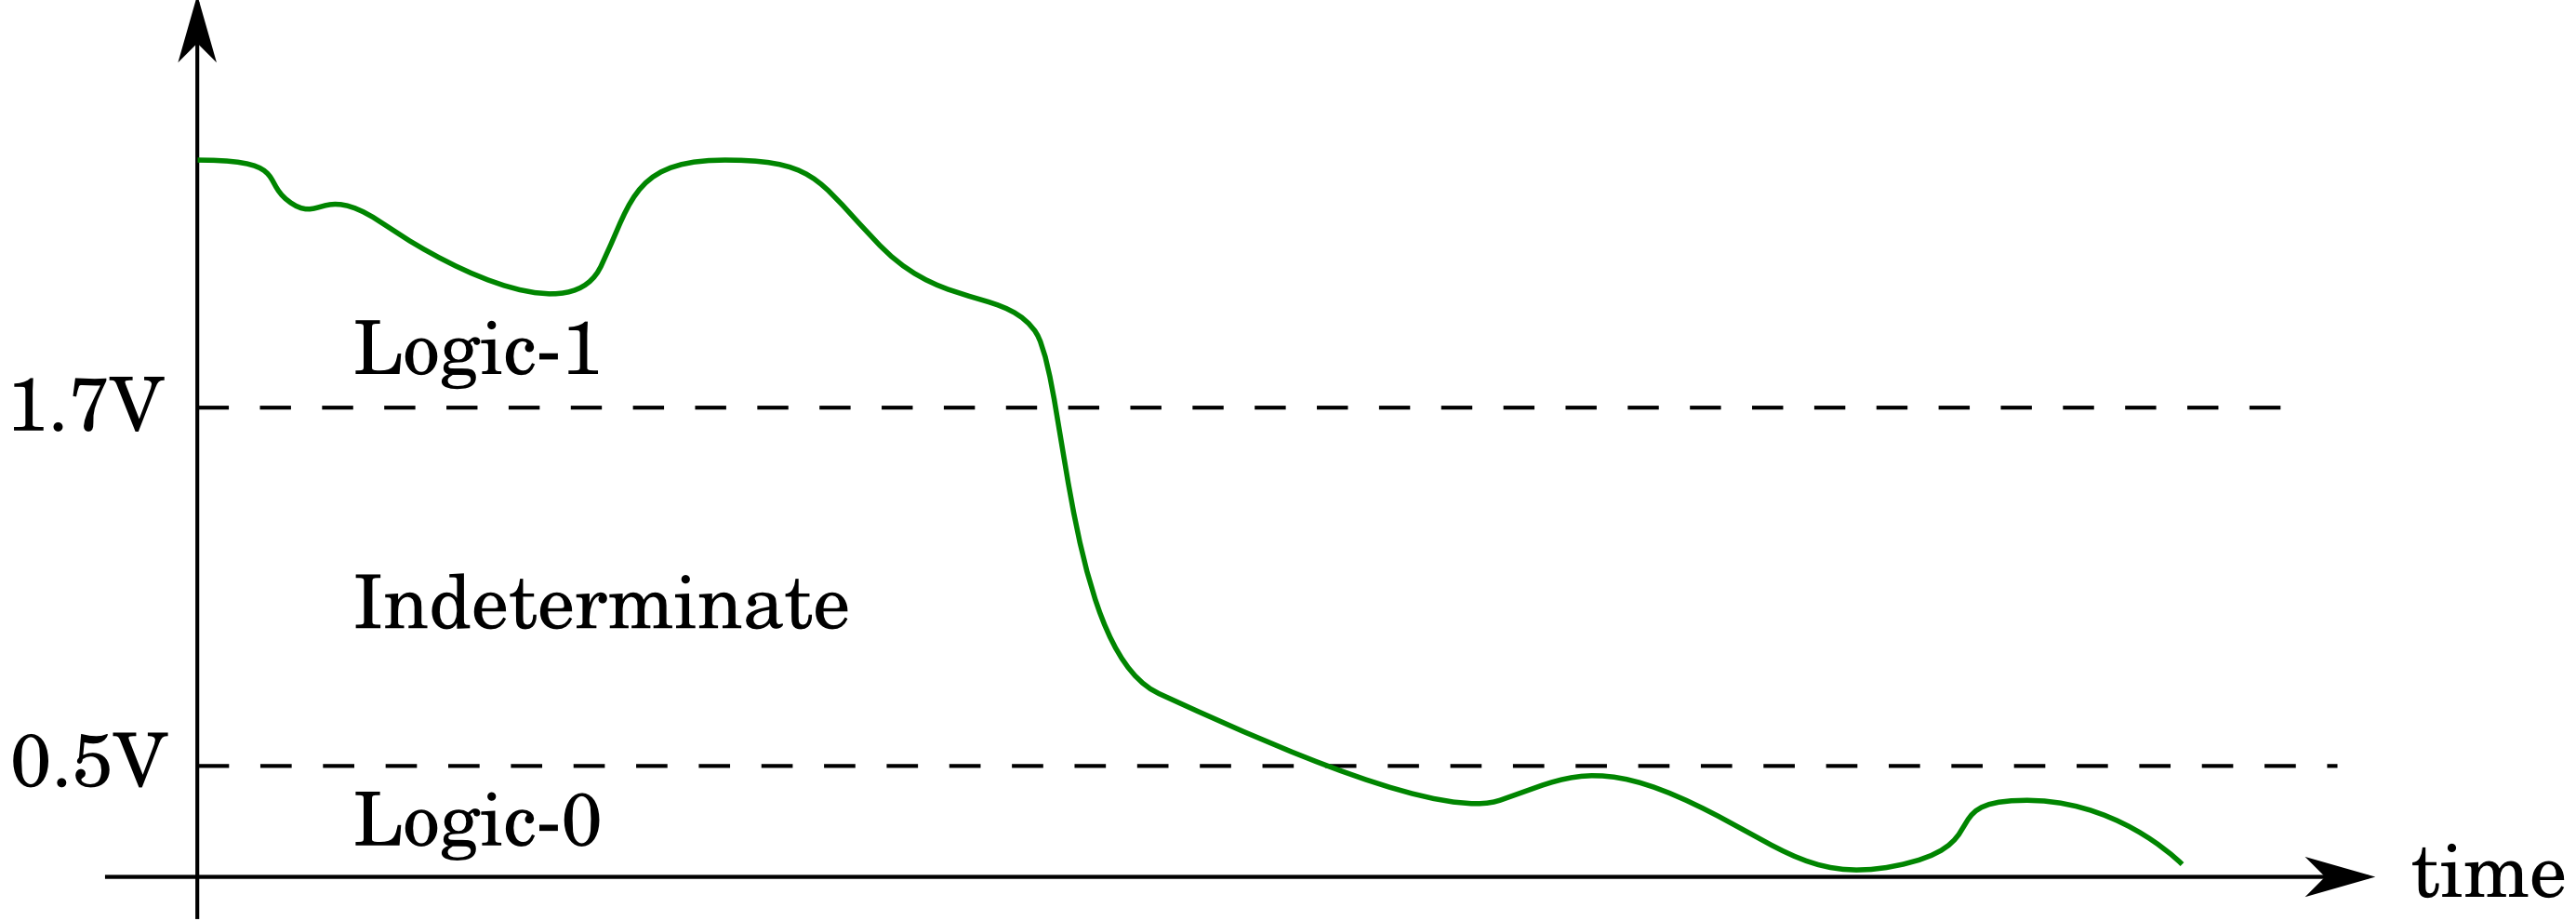
\includegraphics[width=0.3\paperwidth]{img/noise}
\end{figure}



\paragraph{Fan out}

The number of inputs to which the output of a gate is connected.
\begin{itemize}
\item Since $\frac{1}{R}=\frac{1}{R_{1}}+\frac{1}{R_{2}}+\dots+\frac{1}{R_{n}}$
for $n$ resistors in parallel, the load resistance decreases as fan
out increases, so output voltage falls.
\item Slows down circuit since capacitance is summed accross all gates.
\end{itemize}

\section{Synchronous Digital Systems}


\paragraph{Feedback}

Circuit below could:

\begin{figure}[H]
\noindent \centering{}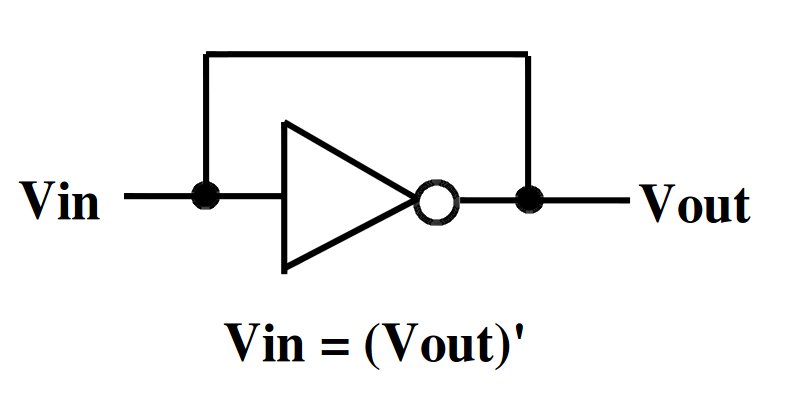
\includegraphics[width=0.1\paperwidth]{img/feedback}
\end{figure}

\begin{itemize}
\item Oscillate between values of 0 and 1.
\item Settle at an intermediate value (actually $\approx$1.2V).
\end{itemize}

\paragraph{The R-S Flip Flop}

E.g. consider:

\begin{figure}[H]
\noindent \centering{}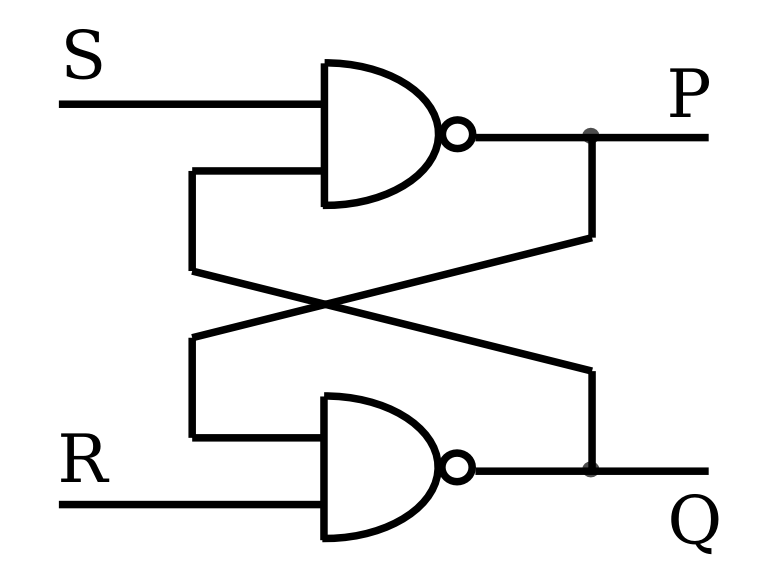
\includegraphics[width=0.1\paperwidth]{img/rs-flipflop}
\end{figure}


By considering all possible states for (RSPQ) and what they lead to
in the following time step:

\begin{figure}[H]
\noindent \centering{}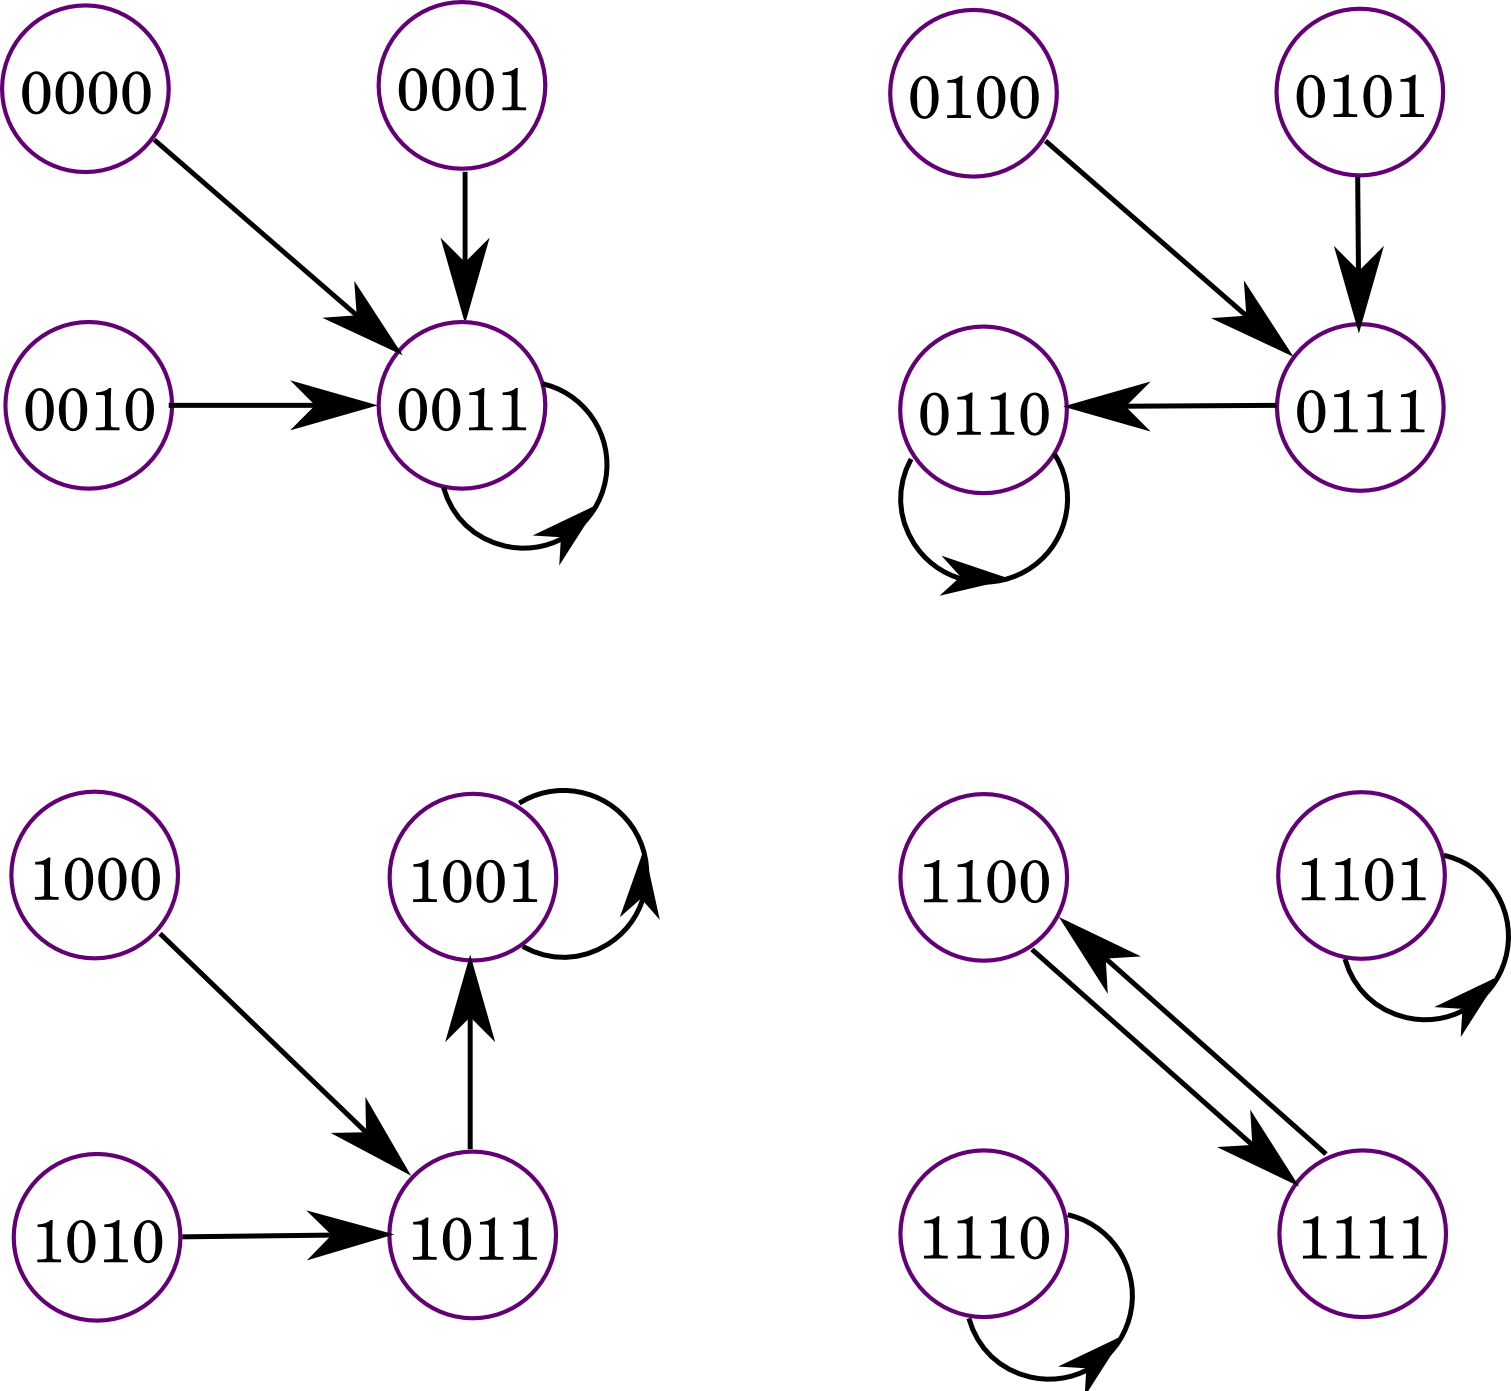
\includegraphics[width=0.25\paperwidth]{img/fsmr}
\end{figure}

\begin{itemize}
\item Uncertain about state at start (until set or reset).
\item SR = 01: \textbf{R}esets memory ($Q$) to 0.
\item SR = 10: \textbf{S}ets memory ($Q$) to 1.
\item SR = 11: Keeps current state.
\end{itemize}

\paragraph{D-Type Latch}

Consider:

\begin{figure}[H]
\noindent \centering{}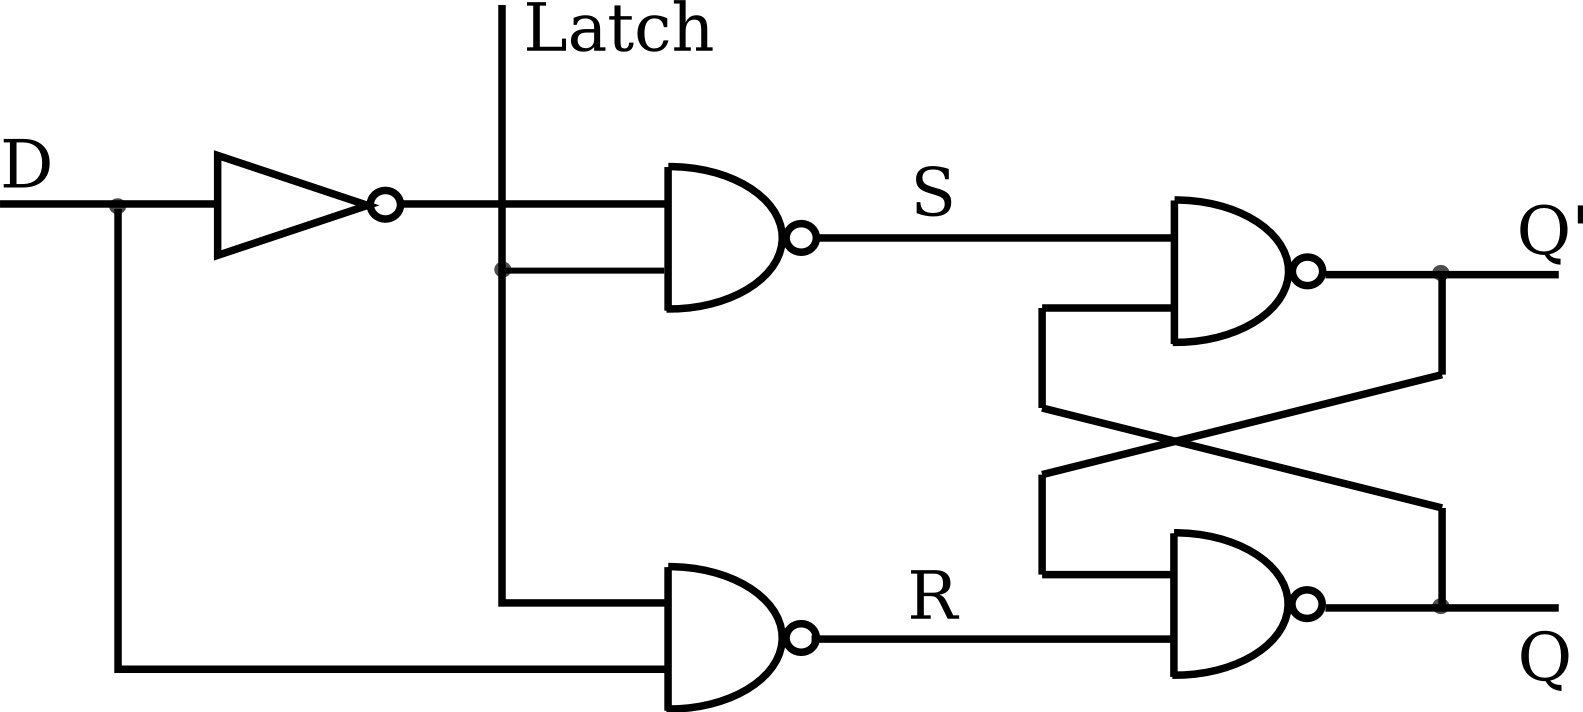
\includegraphics[width=0.2\paperwidth]{img/d-latch}
\end{figure}

\begin{itemize}
\item If latch set to 1, $Q$ becomes $D$.
\item If latch set to 0, $Q$ is held.
\end{itemize}

\paragraph{Edge Triggering}

D-type latch has undesirable behaviour. While latch is 1, any change
on $D$ changes $Q$:

\begin{figure}[H]
\noindent \centering{}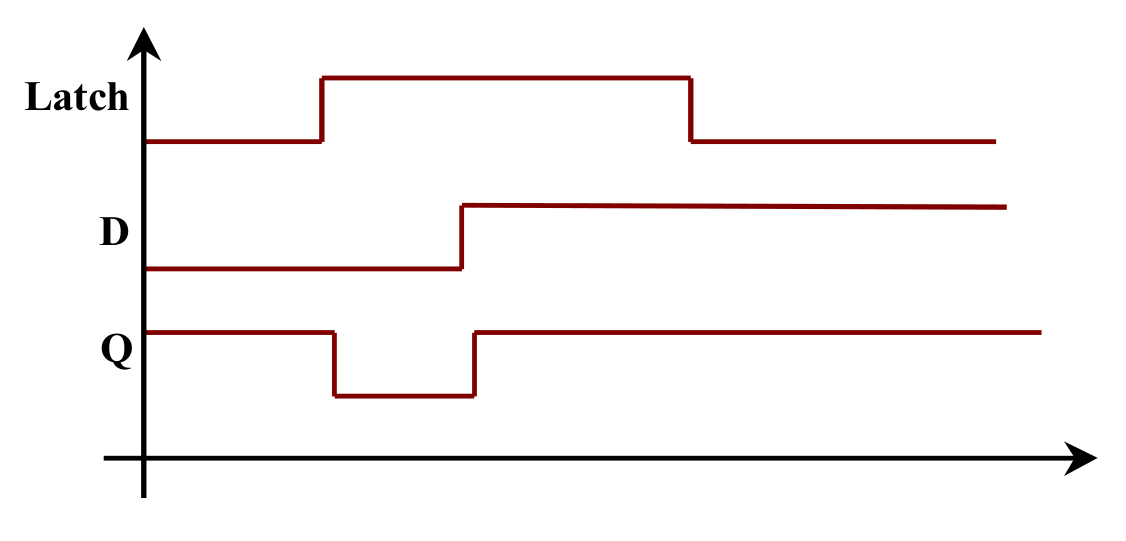
\includegraphics[width=0.2\paperwidth]{img/latch-td}
\end{figure}


\emph{Solution}: edge triggered circuit: Master-Slave Flip-Flop. Now
both gates cannot be open at the same time:

\begin{figure}[H]
\noindent \centering{}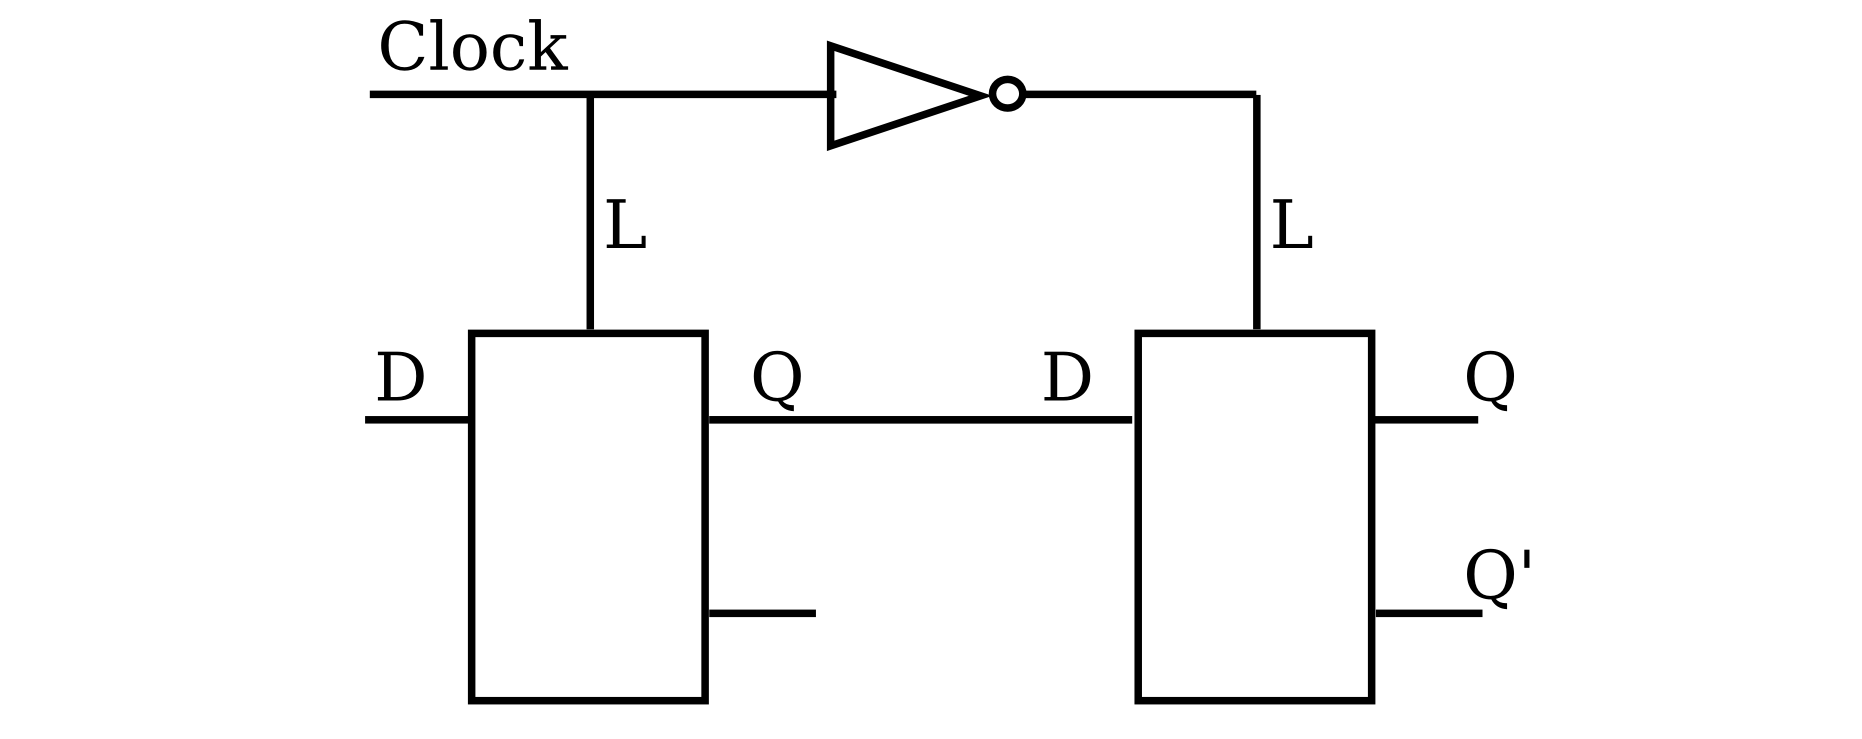
\includegraphics[width=0.2\paperwidth]{img/master-slave}
\end{figure}


\begin{figure}[H]

\paragraph{\noindent Flip-Flops}

Different types:

\noindent \centering{}\subfloat{\noindent \centering{}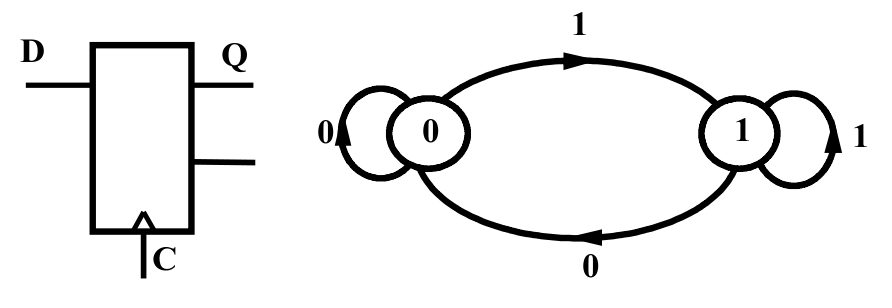
\includegraphics[width=0.15\paperwidth]{img/dq}}
\subfloat{\noindent \centering{}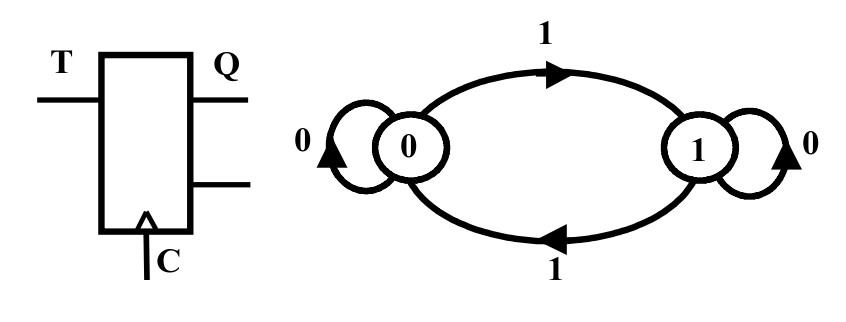
\includegraphics[width=0.15\textwidth]{img/t}}
\subfloat{\noindent \centering{}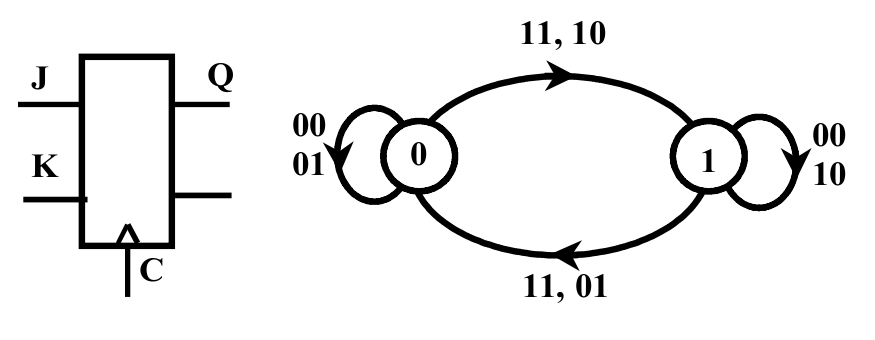
\includegraphics[width=0.15\paperwidth]{img/jk}}
\end{figure}



\paragraph{Preset and Clear}
\begin{itemize}
\item PRESET sets $Q$ to 1.
\item CLEAR sets $Q$ to 0.
\item Behaves normally when PRESET and CLEAR both set to 1.
\end{itemize}
\begin{figure}[H]
\noindent \centering{}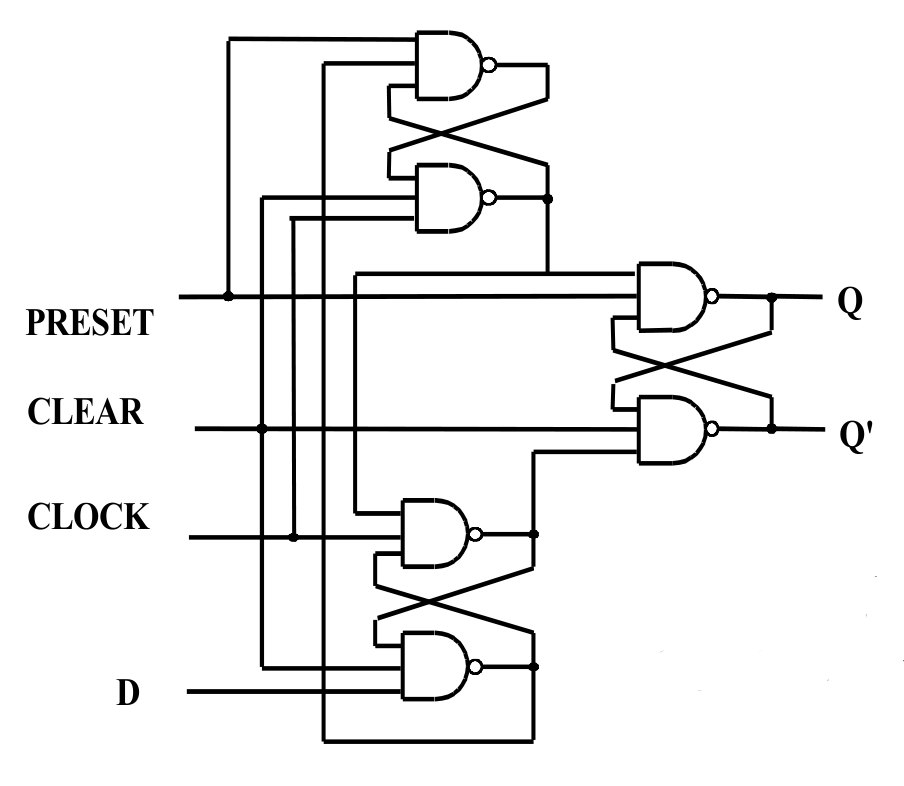
\includegraphics[width=0.2\paperwidth]{img/preset-clear}
\end{figure}



\paragraph{Synchronous Digital Systems}
\begin{itemize}
\item \emph{Synchronous}: Circuit only changes in response to system clock.
\item \emph{Sequential}: Goes through sequence of states.
\end{itemize}
\emph{General form}: 
\begin{figure}[H]
\noindent \centering{}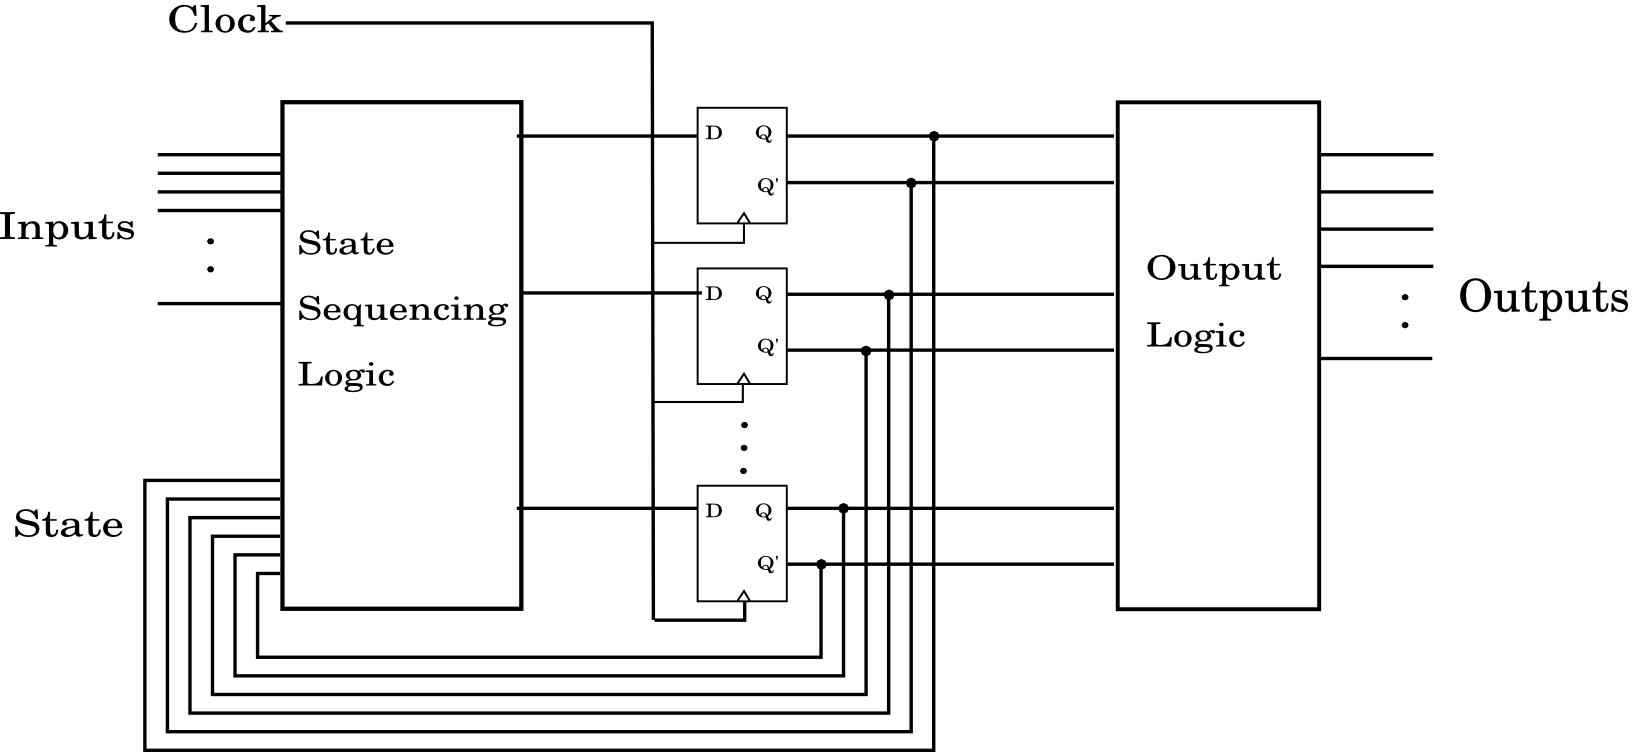
\includegraphics[width=0.3\paperwidth]{img/seqcircuit}
\end{figure}

\begin{itemize}
\item The state sequencing logic and output logic are combinatorial circuits.
\item Outputs depend only on state of circuit.
\item Next state depends on current state and inputs.
\end{itemize}

\paragraph{Sequential Circuit \emph{Design Process}}
\begin{enumerate}
\item Determine the required number of states and assign each output to
a state. State assignments should be adjacent (i.e. only changing 1 digit, 011 \textrightarrow{} 111) if they:

\begin{enumerate}
\item Have the same next state for a given input.
\item Are the next states of the same state.
\item \emph{Or choose to minimise output logic.}
\end{enumerate}
\item Determine the state transitions. Draw a state transition diagram and
a state transition table.
\item For each flip-flop input $D_{n}$, draw a Karnaugh Map and determine
a Boolean expression in terms of the flip-flop outputs and circuit
inputs. Simplify.
\item Check don't cares. Fix by one of these methods:

\begin{enumerate}
\item Look at K-Maps and try to find a simple modification.
\item Include unused states and redo.
\end{enumerate}
\item Determine Boolean expressions for output from the state assignments,
using Karnaugh maps.
\item Draw and optimise the circuit. Remember common terms only need to
be committed to hardware once!
\end{enumerate}

\section{Functional Design}


\paragraph{Shift Registers}
\begin{itemize}
\item Inside a computer data is organised in a parallel form, but communication
usually involves serial data.
\item Registers are an ordered group of flip-flops connected to a single
clock.
\item We can convert paralell and serial data.
\end{itemize}
\begin{figure}[H]
\noindent \centering{}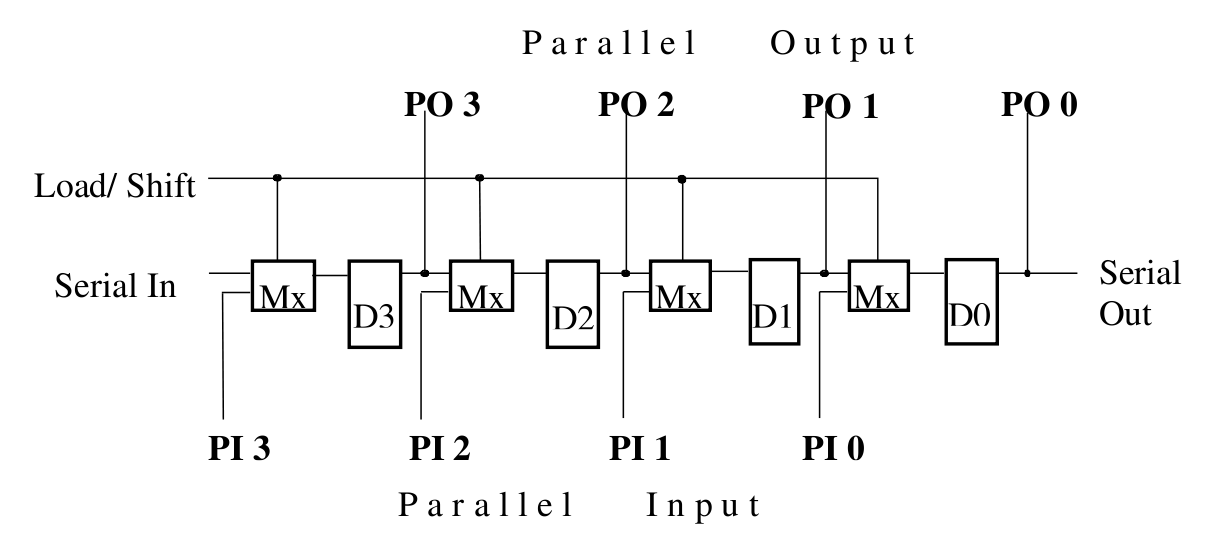
\includegraphics[width=0.35\paperwidth]{img/register}
\end{figure}

\begin{itemize}
\item Time to load a parallel input depends on length of register.
\item Requires a seperate (slower) clock to processor clock.
\end{itemize}

\paragraph{Multi-Function Registers}

Want to be able to shift bits left / right with the same circuitry.

\begin{figure}[H]
\noindent \centering{}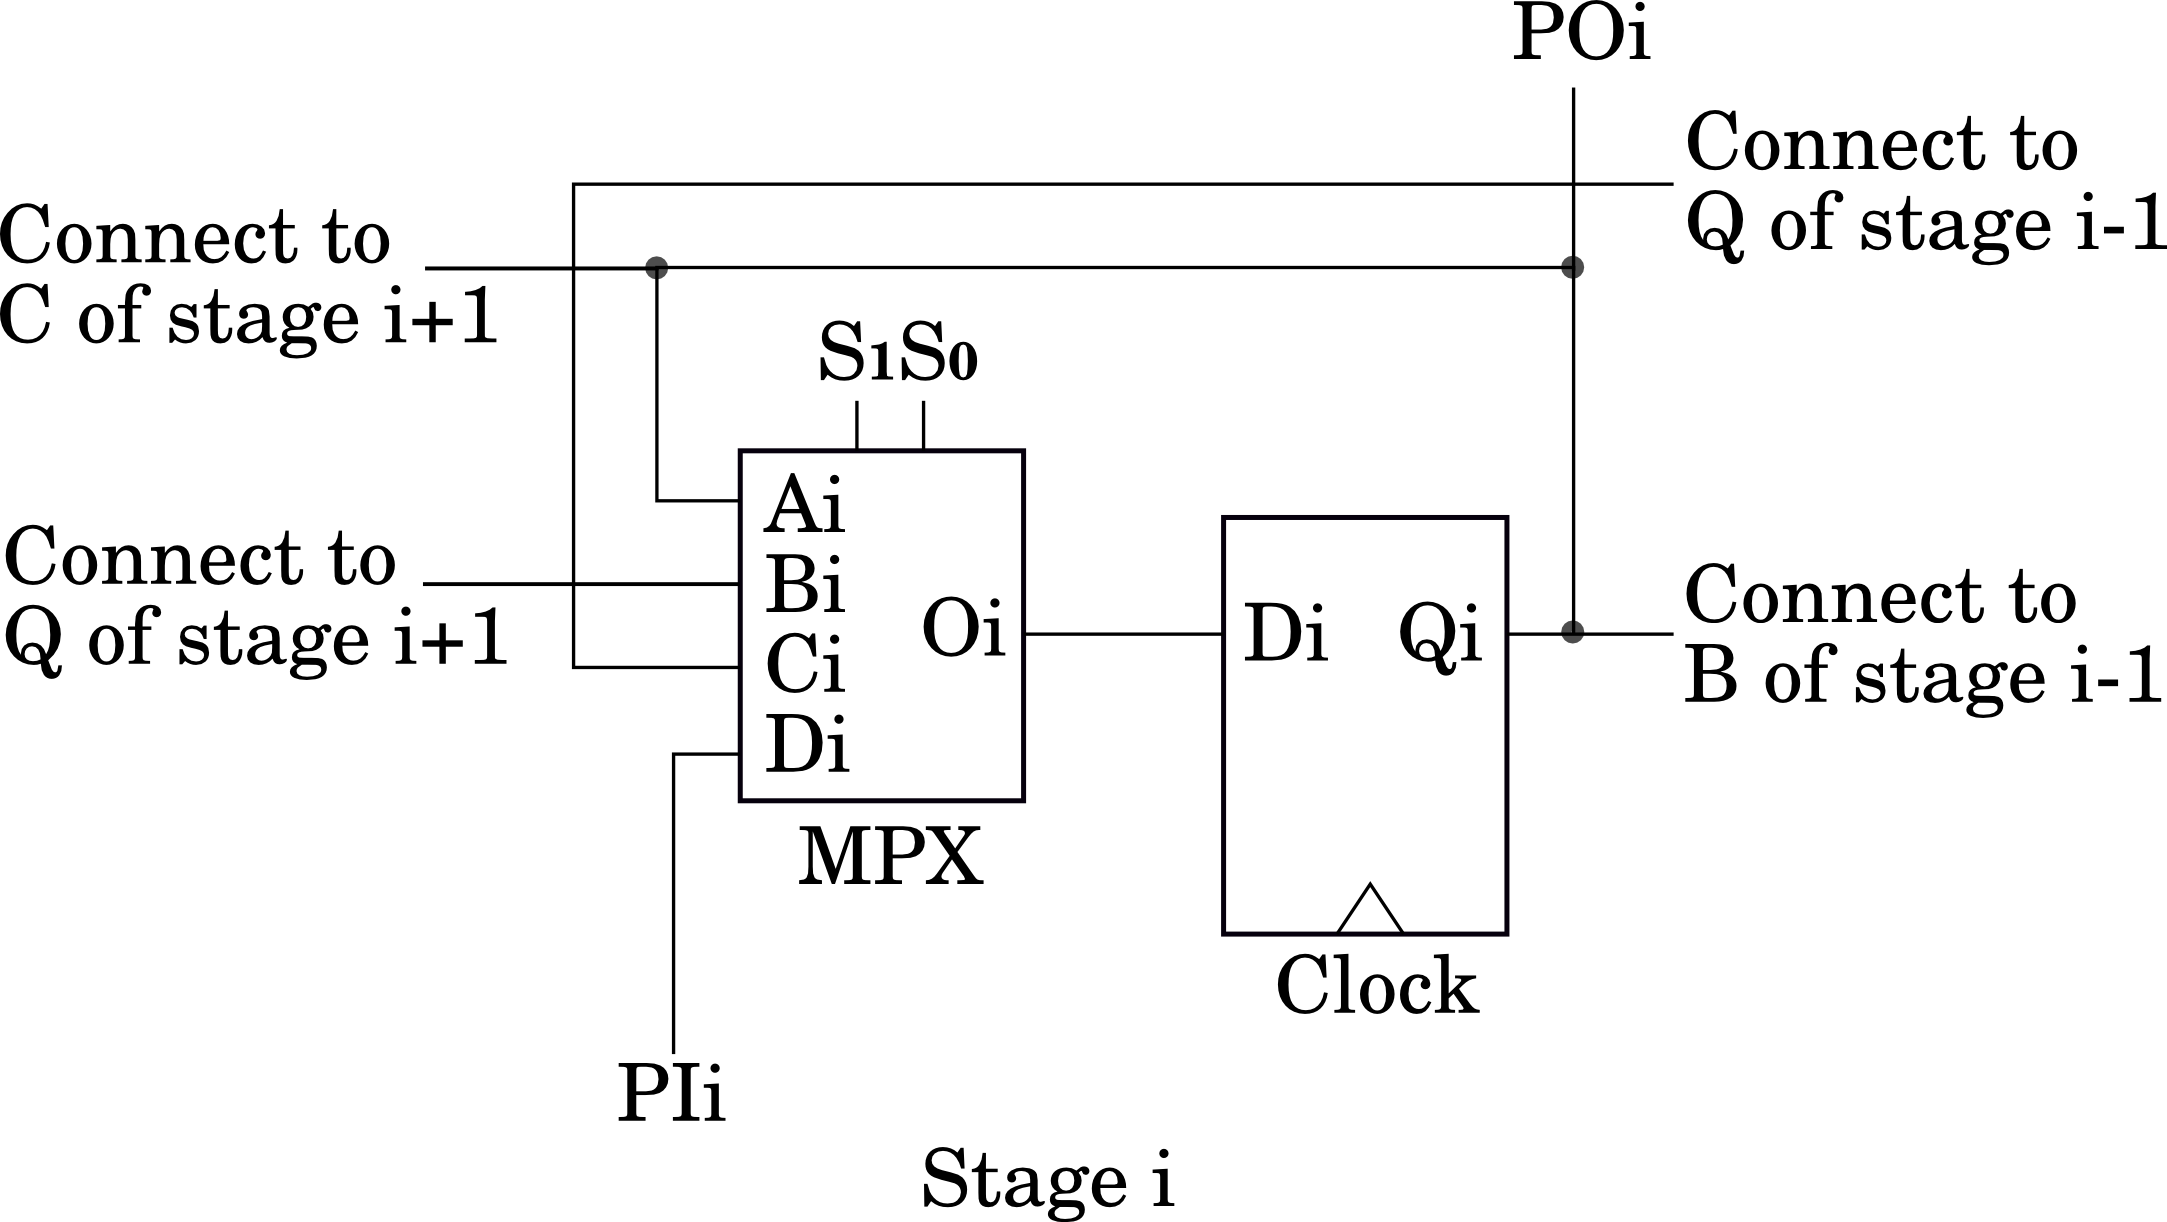
\includegraphics[width=0.3\paperwidth]{img/mfregister}
\end{figure}


Here we can use 00 to hold, 01 to shift right, 10 to shift left, 11
to load parallel.


\paragraph{Dividing Clocks}

We can divide clocks by 2 easily:

\begin{figure}[H]
\noindent \centering{}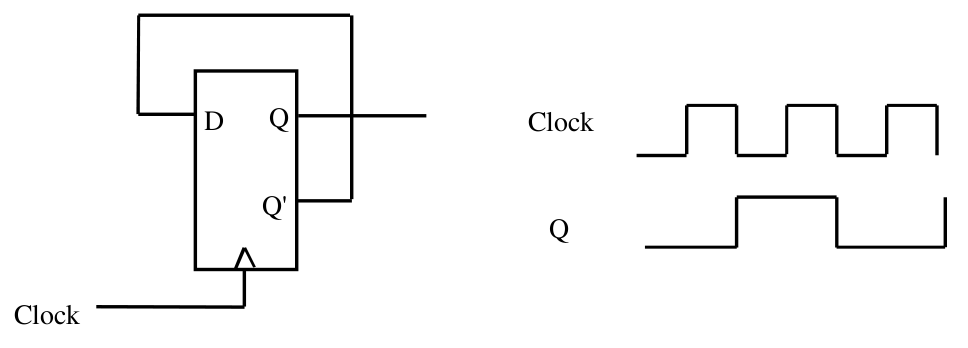
\includegraphics[width=0.25\paperwidth]{img/clockdiv2}
\end{figure}


We can stack these, one after the other, to divide by any power of
2.

For non-powers of 2, we:
\begin{itemize}
\item Design to the next highest power of 2.
\item Then use clear when the required count is reached to reset count to
0.
\end{itemize}
E.g. for 5:

\begin{figure}[H]
\noindent \centering{}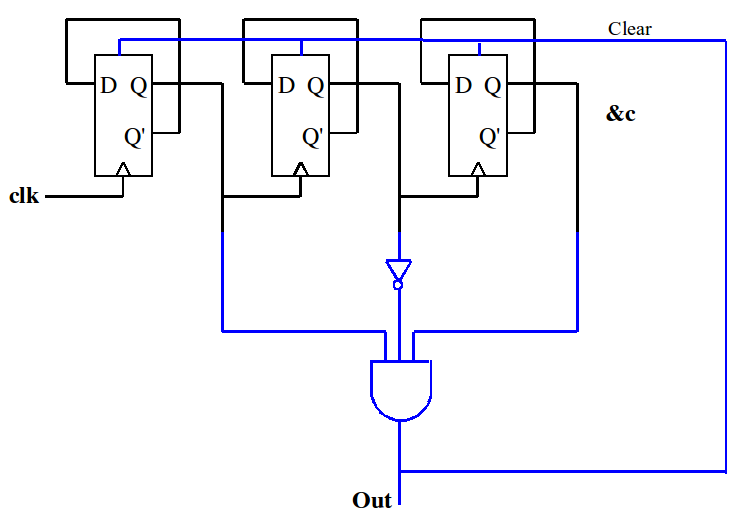
\includegraphics[width=0.225\paperwidth]{img/clockdiv5}
\end{figure}



\paragraph{Register Transfer Operations}

($R_{\mbox{dst}}\leftarrow R_{\mbox{src}}$)

\begin{figure}[H]
\noindent \centering{}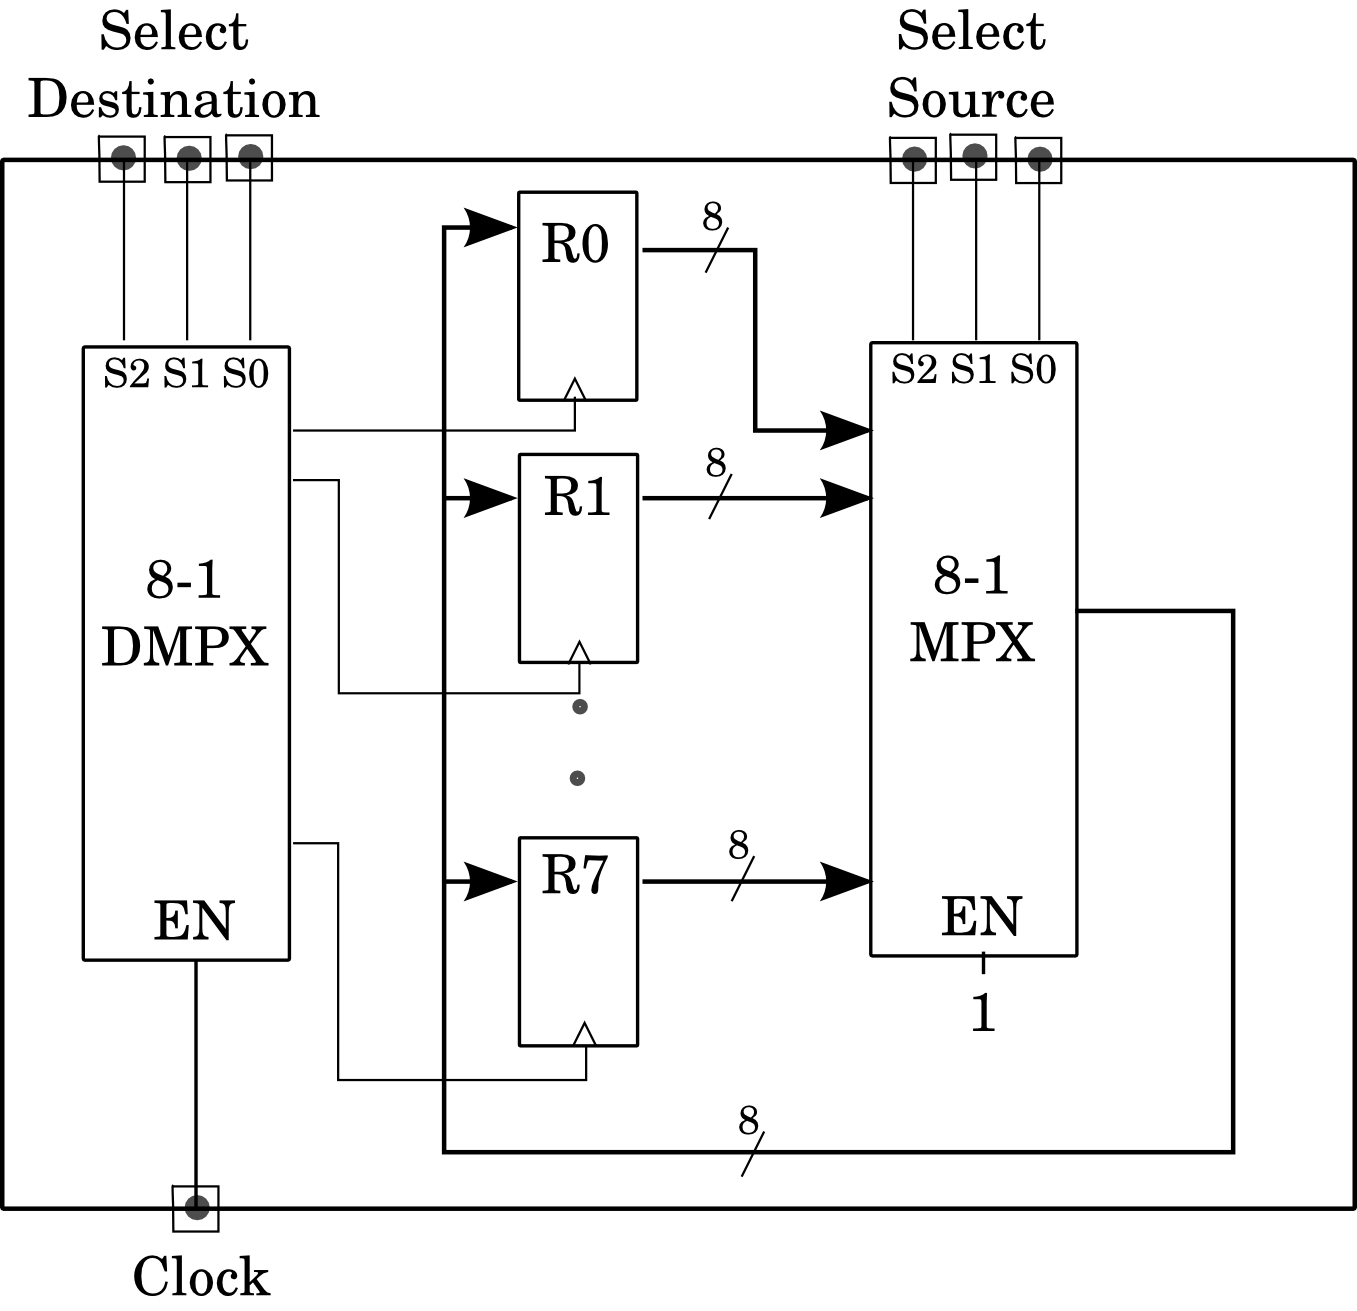
\includegraphics[width=0.225\paperwidth]{img/reg-transfer}
\end{figure}

\begin{enumerate}
\item Select source register using multiplexer.
\item Select destination register using demultiplexer.
\item Transfer data from source to destination.
\end{enumerate}

\paragraph{Multiplexers}

A 4-to-1 multiplexer:

\begin{figure}[H]
\noindent \centering{}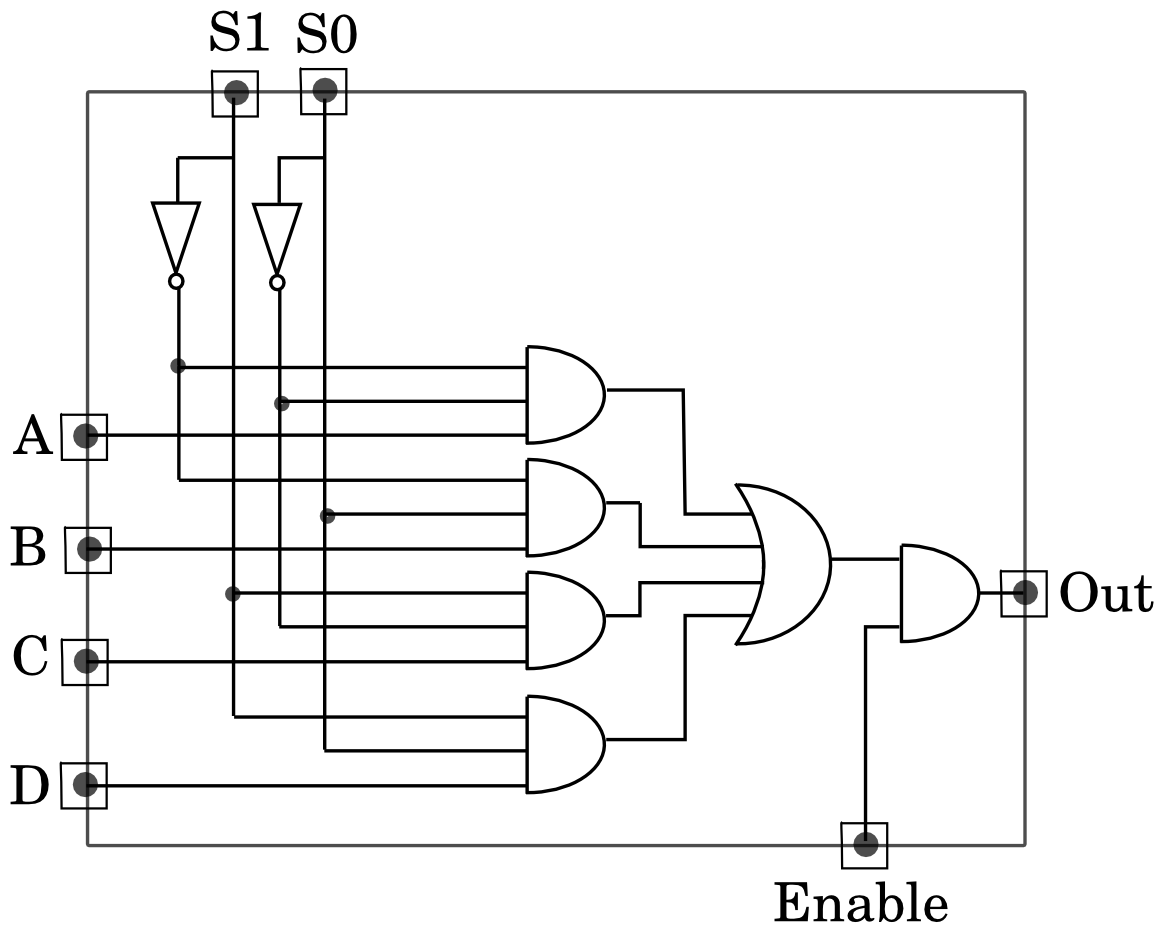
\includegraphics[width=0.15\paperwidth]{img/mx4}
\end{figure}


Extended to 8-to-1 by functional design:

\begin{figure}[H]
\noindent \centering{}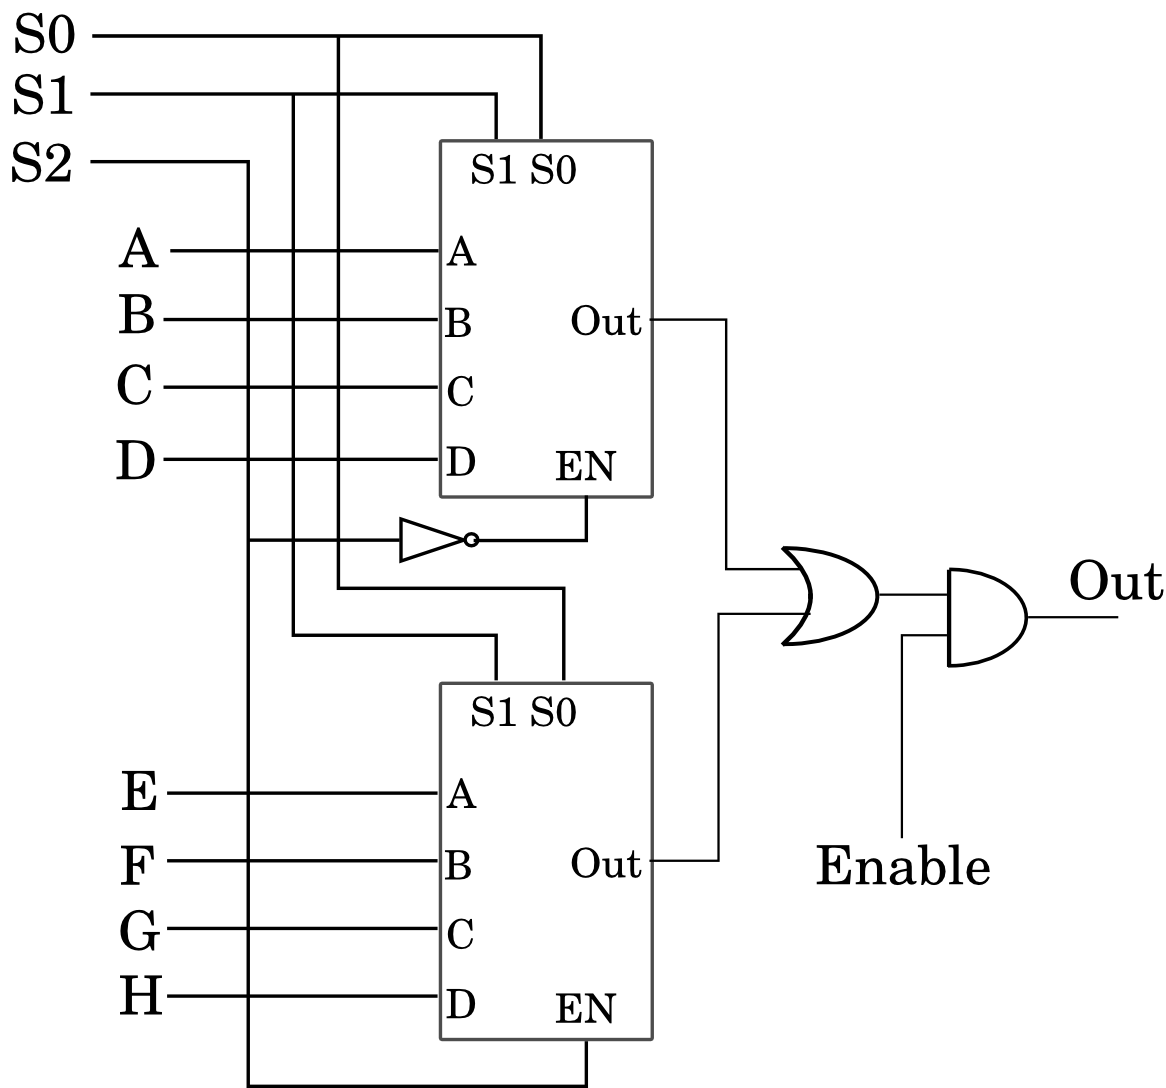
\includegraphics[width=0.2\paperwidth]{img/mx8}
\end{figure}



\paragraph{Demultiplexers}

A 2-to-4 demultiplexer:

\begin{figure}[H]
\noindent \centering{}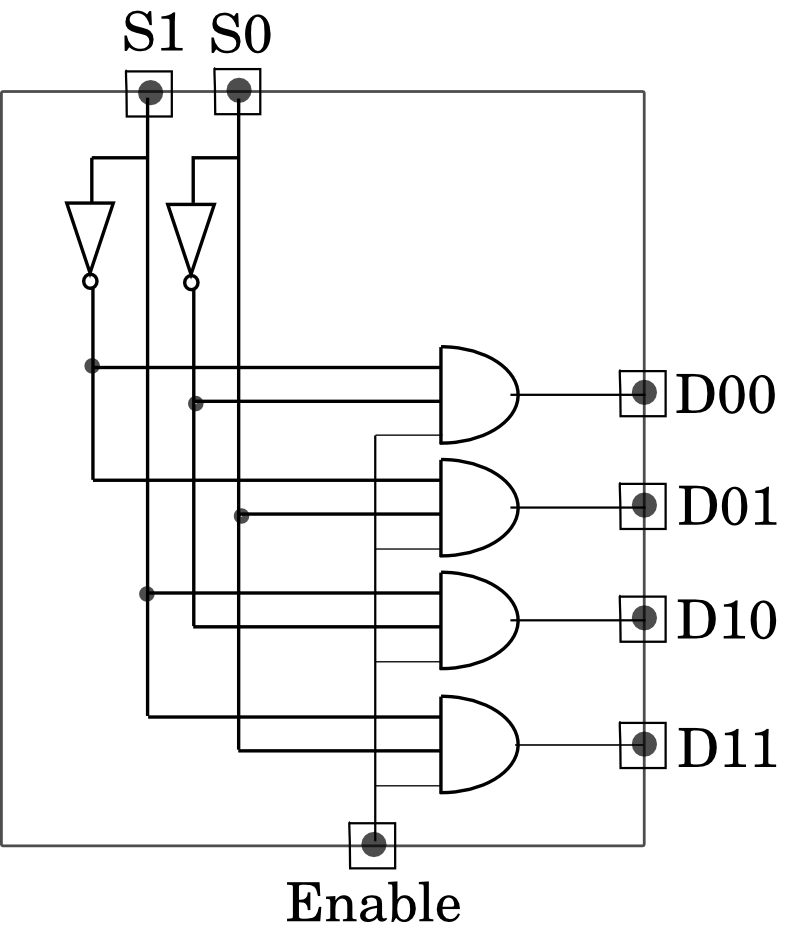
\includegraphics[width=0.125\paperwidth]{img/dmx4}
\end{figure}


Extended to 3-to-8 by functional design:

\begin{figure}[H]
\noindent \centering{}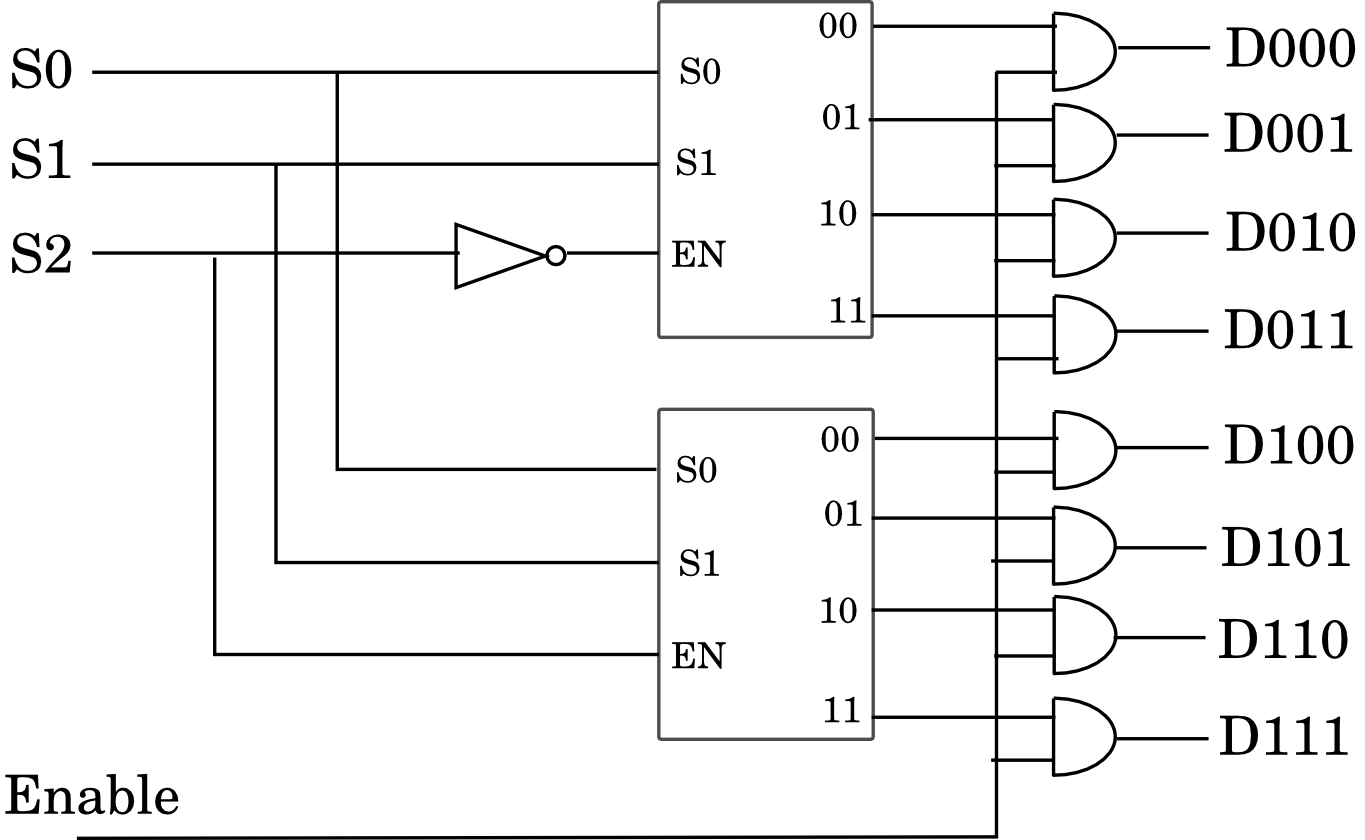
\includegraphics[width=0.2\paperwidth]{img/dmx8}
\end{figure}



\paragraph{Comparators}

A 1-bit comparator:

\begin{figure}[H]
\noindent \centering{}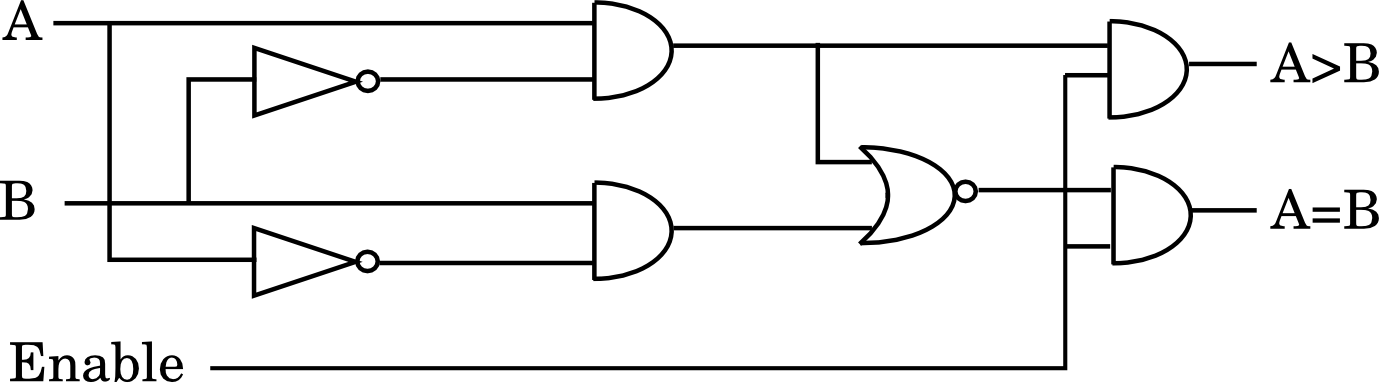
\includegraphics[width=0.2\paperwidth]{img/comparator1}
\end{figure}


Extended to 4-bit by functional design:

\begin{figure}[H]
\noindent \centering{}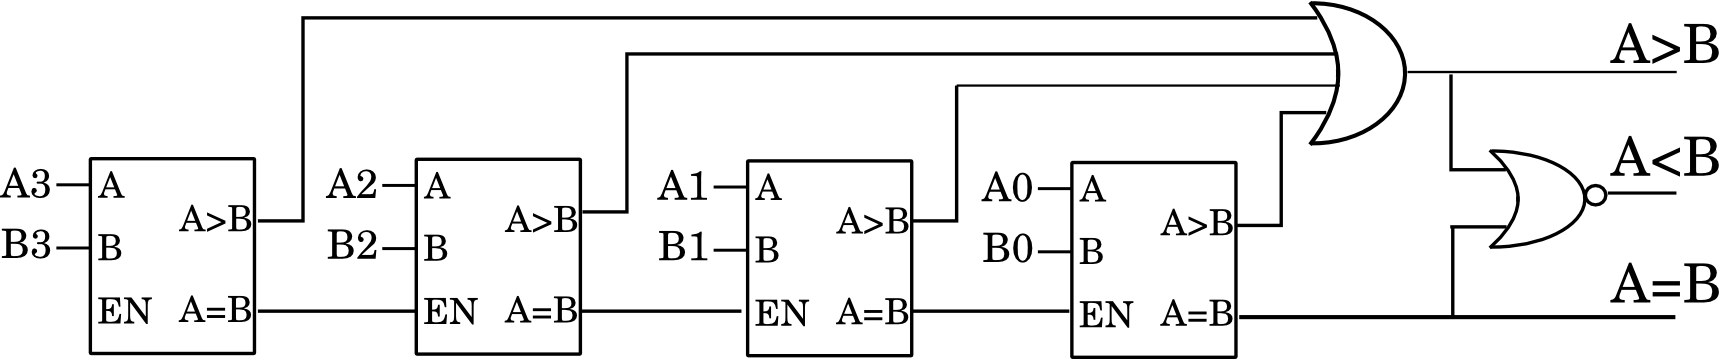
\includegraphics[width=0.25\paperwidth]{img/comparator4}
\end{figure}



\subsection{Computer Arithmetic}


\paragraph{Half Adder}

$S=A\oplus B$ and $C=A\cdot B$:

\begin{table}[H]
\noindent \begin{minipage}[t]{0.25\textwidth}

\noindent \begin{centering}
\subfloat{\noindent \centering{}%
\begin{tabular}{cccc}
\toprule 
{\footnotesize{}A} & {\footnotesize{}B} & \textbf{\footnotesize{}Sum} & \textbf{\footnotesize{}Carry}\tabularnewline
\midrule
{\footnotesize{}0} & {\footnotesize{}0} & \textbf{\footnotesize{}0} & \textbf{\footnotesize{}0}\tabularnewline
{\footnotesize{}0} & {\footnotesize{}1} & \textbf{\footnotesize{}1} & \textbf{\footnotesize{}0}\tabularnewline
{\footnotesize{}1} & {\footnotesize{}0} & \textbf{\footnotesize{}1} & \textbf{\footnotesize{}0}\tabularnewline
{\footnotesize{}1} & {\footnotesize{}1} & \textbf{\footnotesize{}0} & \textbf{\footnotesize{}1}\tabularnewline
\bottomrule
\end{tabular}}
\par\end{centering}

\noindent \end{minipage}
\begin{minipage}[c]{0.25\textwidth}

\noindent \begin{centering}
\subfloat{\noindent \centering{}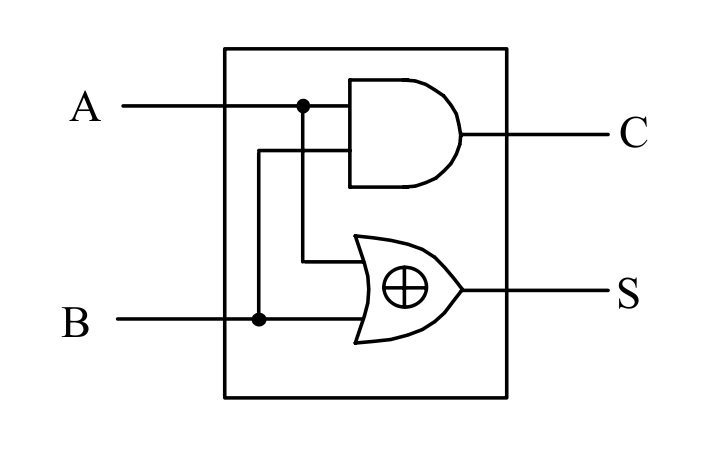
\includegraphics[width=0.15\paperwidth]{img/halfadder}}
\par\end{centering}

\noindent \centering{}\end{minipage}
\end{table}



\paragraph{Full Adder}

Need to propogate the carry, $S=A\oplus B\oplus C$ and $C_{\mbox{out}}=C\cdot\left(A\oplus B\right)+A\cdot B$.

\begin{table}[H]
\noindent \begin{minipage}[t]{0.25\textwidth}

\noindent \begin{centering}
\subfloat{\noindent \centering{}%
\begin{tabular}{ccccc}
\toprule 
{\footnotesize{}A} & {\footnotesize{}B} & {\footnotesize{}$\mbox{C}_{\mbox{in}}$} & \textbf{\footnotesize{}S} & {\footnotesize{}$\mbox{\textbf{C}}_{\mbox{out}}$}\tabularnewline
\midrule
{\footnotesize{}0} & {\footnotesize{}0} & {\footnotesize{}0} & \textbf{\footnotesize{}0} & \textbf{\footnotesize{}0}\tabularnewline
{\footnotesize{}0} & {\footnotesize{}0} & {\footnotesize{}1} & \textbf{\footnotesize{}1} & \textbf{\footnotesize{}0}\tabularnewline
{\footnotesize{}0} & {\footnotesize{}1} & {\footnotesize{}0} & \textbf{\footnotesize{}1} & \textbf{\footnotesize{}0}\tabularnewline
{\footnotesize{}0} & {\footnotesize{}1} & {\footnotesize{}1} & \textbf{\footnotesize{}0} & \textbf{\footnotesize{}1}\tabularnewline
\midrule
{\footnotesize{}1} & {\footnotesize{}0} & {\footnotesize{}0} & \textbf{\footnotesize{}1} & \textbf{\footnotesize{}0}\tabularnewline
{\footnotesize{}1} & {\footnotesize{}0} & {\footnotesize{}1} & \textbf{\footnotesize{}0} & \textbf{\footnotesize{}1}\tabularnewline
{\footnotesize{}1} & {\footnotesize{}1} & {\footnotesize{}0} & \textbf{\footnotesize{}0} & \textbf{\footnotesize{}1}\tabularnewline
{\footnotesize{}1} & {\footnotesize{}1} & {\footnotesize{}1} & \textbf{\footnotesize{}1} & \textbf{\footnotesize{}1}\tabularnewline
\bottomrule
\end{tabular}}
\par\end{centering}

\noindent \end{minipage}
\begin{minipage}[c]{0.25\textwidth}

\subfloat{\noindent \centering{}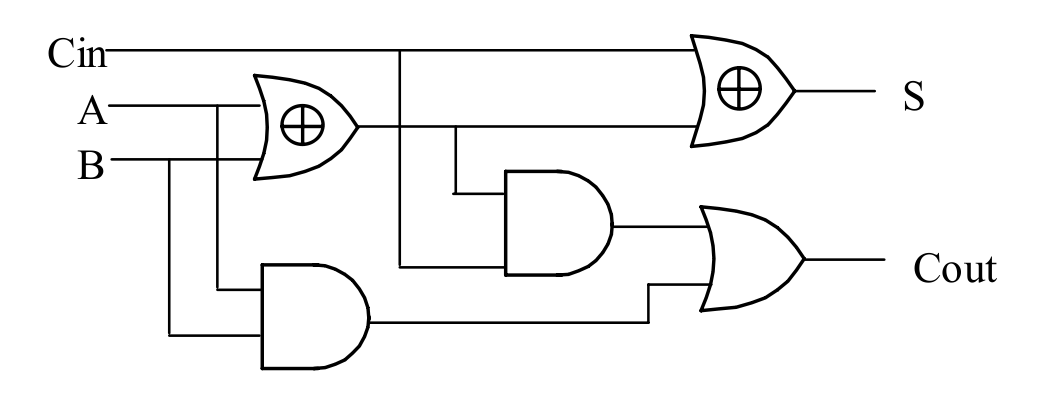
\includegraphics[width=0.2\paperwidth]{img/fulladder}}

\noindent \centering{}\end{minipage}
\end{table}



\paragraph{\noindent Ripple Through Carry Adder}

For $n$ bits:

\begin{figure}[H]
\noindent \centering{}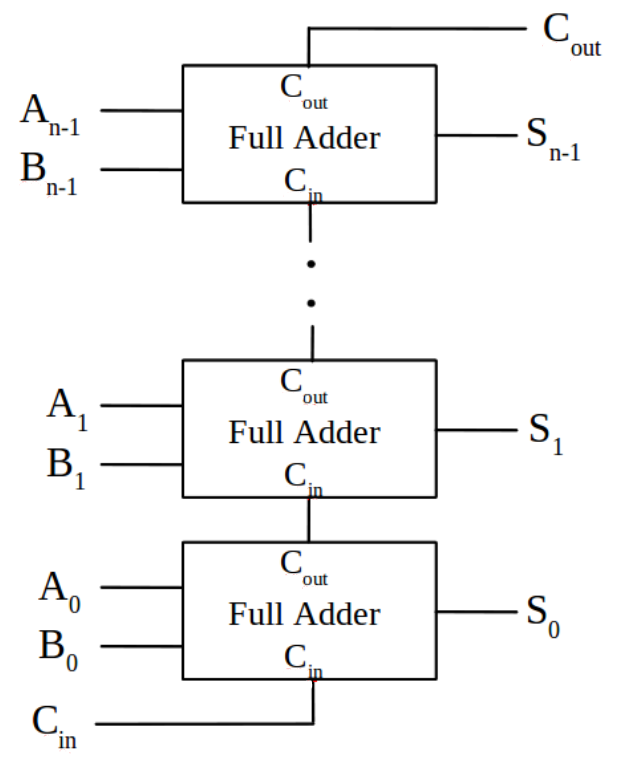
\includegraphics[width=0.15\paperwidth]{img/ripplethroughadder}
\end{figure}



\paragraph{Serial Adder}

Assumes bits arrive least significant first.

\begin{figure}[H]
\noindent \centering{}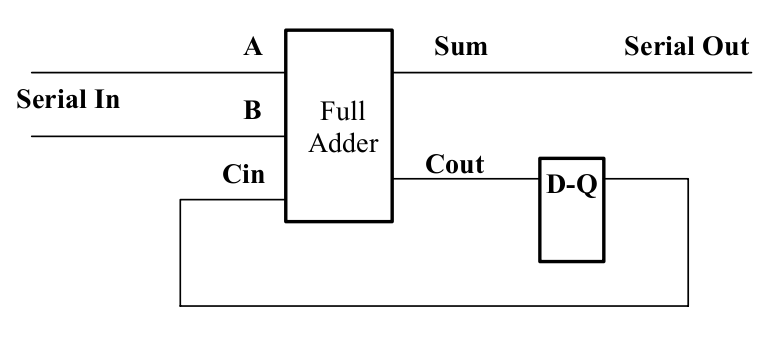
\includegraphics[width=0.2\paperwidth]{img/serialadder}
\end{figure}



\paragraph{Subtractor}

Difference $=A\oplus B\oplus P$ and Borrow $=A'\cdot (B\oplus P) + B\cdot P$:

\begin{table}[H]
\noindent \begin{minipage}[t]{0.25\textwidth}

\noindent \begin{centering}
\subfloat{\noindent \centering{}%
\begin{tabular}{ccccc}
\toprule 
{\footnotesize{}A} & {\footnotesize{}B} & {\footnotesize{}P} & \textbf{\footnotesize{}Difference} & \textbf{\footnotesize{}Borrow}\tabularnewline
\midrule
{\footnotesize{}0} & {\footnotesize{}0} & {\footnotesize{}0} & \textbf{\footnotesize{}0} & \textbf{\footnotesize{}0}\tabularnewline
{\footnotesize{}0} & {\footnotesize{}1} & {\footnotesize{}0} & \textbf{\footnotesize{}1} & \textbf{\footnotesize{}1}\tabularnewline
{\footnotesize{}1} & {\footnotesize{}0} & {\footnotesize{}0} & \textbf{\footnotesize{}1} & \textbf{\footnotesize{}0}\tabularnewline
{\footnotesize{}1} & {\footnotesize{}1} & {\footnotesize{}0} & \textbf{\footnotesize{}0} & \textbf{\footnotesize{}0}\tabularnewline
\midrule
{\footnotesize{}0} & {\footnotesize{}0} & {\footnotesize{}1} & \textbf{\footnotesize{}1} & \textbf{\footnotesize{}1}\tabularnewline
{\footnotesize{}0} & {\footnotesize{}1} & {\footnotesize{}1} & \textbf{\footnotesize{}0} & \textbf{\footnotesize{}1}\tabularnewline
{\footnotesize{}1} & {\footnotesize{}0} & {\footnotesize{}1} & \textbf{\footnotesize{}0} & \textbf{\footnotesize{}0}\tabularnewline
{\footnotesize{}1} & {\footnotesize{}1} & {\footnotesize{}1} & \textbf{\footnotesize{}1} & \textbf{\footnotesize{}1}\tabularnewline
\bottomrule
\end{tabular}}
\par\end{centering}

\noindent \end{minipage}
\begin{minipage}[c]{0.25\textwidth}

\subfloat{\noindent \centering{}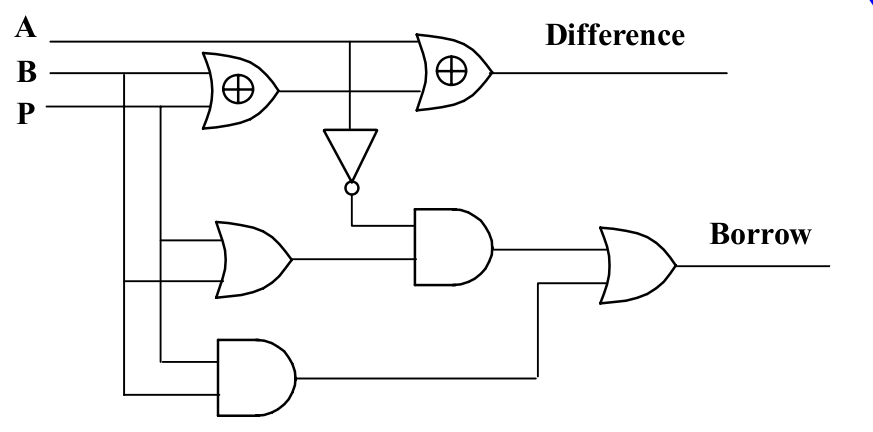
\includegraphics[width=0.2\paperwidth]{img/subtractor}}

\noindent \centering{}\end{minipage}
\end{table}



\paragraph{Subtractor using Two's Complement}

$A-B=A+\left(-B\right)$.

\begin{figure}[H]
\noindent \centering{}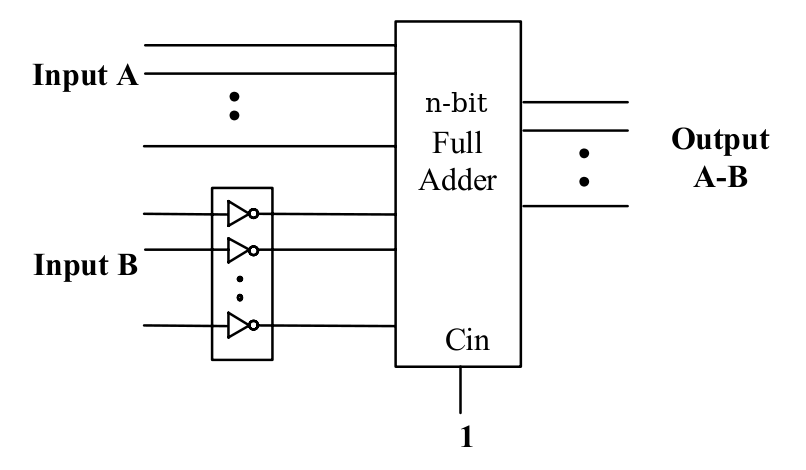
\includegraphics[width=0.2\paperwidth]{img/twocomplement-sub}
\end{figure}



\paragraph{Multiplication}

$a_{1}a_{0}\times b_{1}b_{0}=a_{1}\cdot b_{1}\cdot2^{2}+a_{0}\cdot b_{1}\cdot2+a_{1}\cdot b_{0}\cdot2+a_{0}\cdot b_{0}$.
Multiplication by 2 is equivalent to a left shift, so for 2 bits:

\begin{figure}[H]
\noindent \centering{}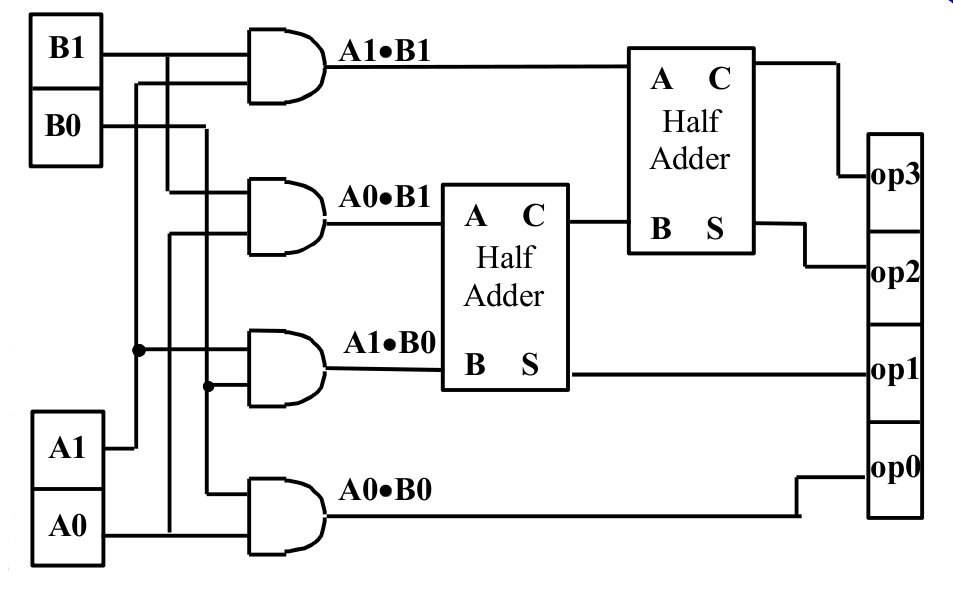
\includegraphics[width=0.25\paperwidth]{img/multiply2}
\end{figure}


Using functional design, for 4 bits:

\begin{figure}[H]
\noindent \centering{}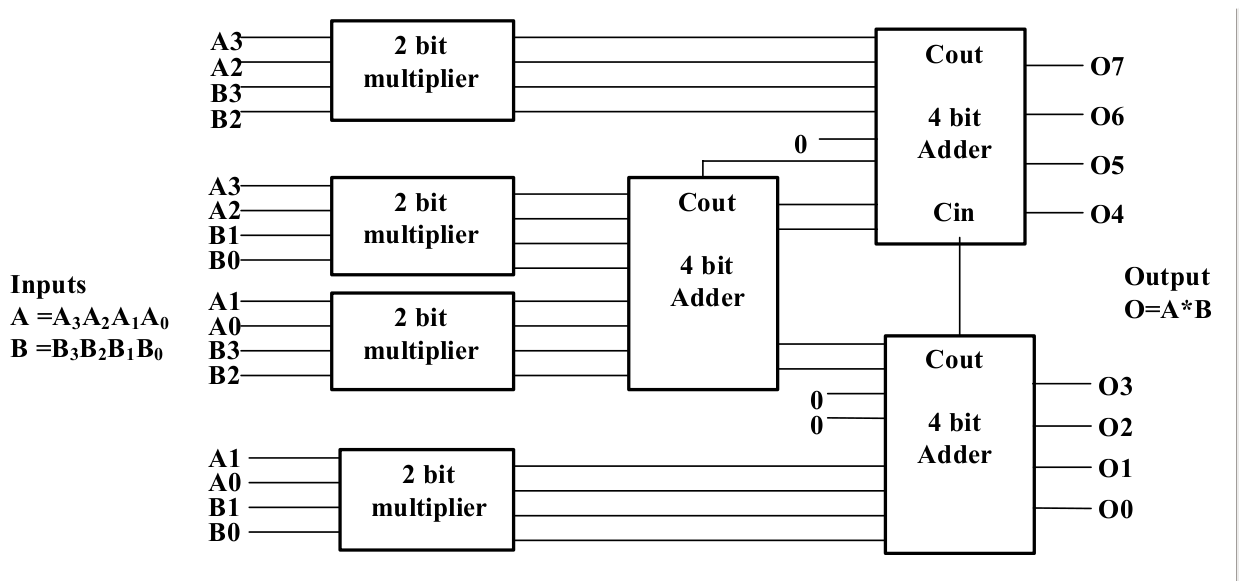
\includegraphics[width=0.35\paperwidth]{img/multiply4}
\end{figure}



\paragraph{Division}
\begin{itemize}
\item Can be done procedurally using shifts and subtracts.
\item Combinatorial hardware also exists.
\end{itemize}

\paragraph{The ALU}

A simple combinatorial circuit that bundles together arithmetic circuits:

\begin{figure}[H]
\noindent \centering{}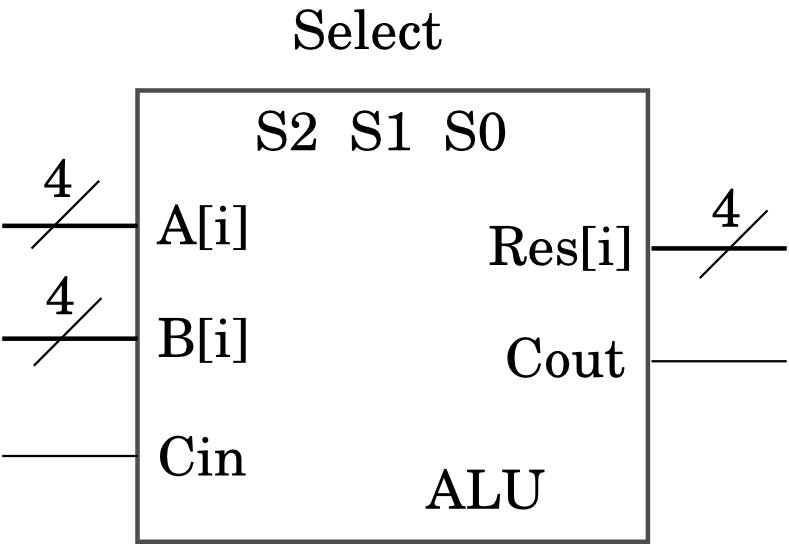
\includegraphics[width=0.125\paperwidth]{img/alu}
\end{figure}


Requires two multiplexers per bit. Assuming the two subtractors and
one adder are already in place:

\begin{table}[H]
\noindent \begin{minipage}[t]{0.25\textwidth}

\noindent \begin{centering}
\subfloat{\noindent \centering{}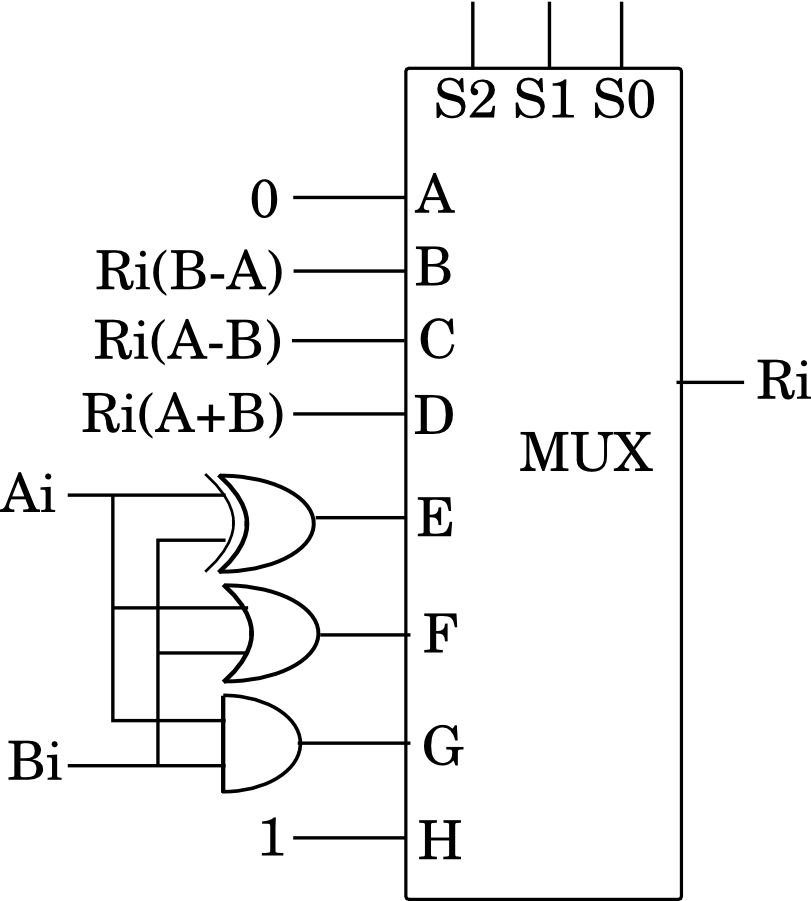
\includegraphics[width=0.125\paperwidth]{img/alu1}}
\par\end{centering}

\noindent \end{minipage}
\begin{minipage}[t]{0.25\textwidth}

\noindent \begin{centering}
\subfloat{\noindent \centering{}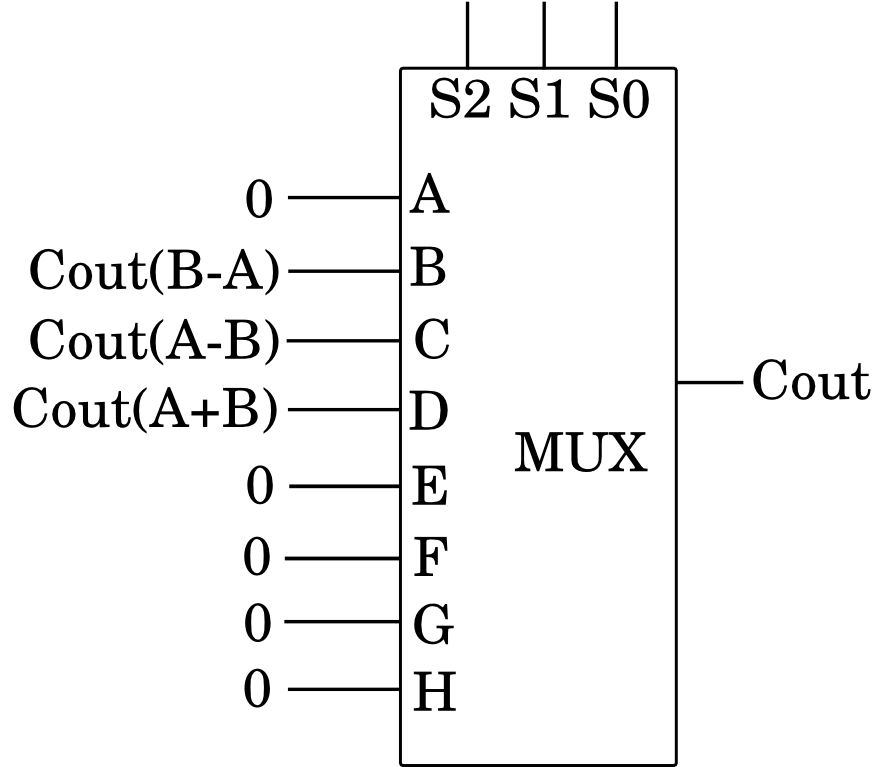
\includegraphics[width=0.15\paperwidth]{img/alu2}}
\par\end{centering}

\noindent \centering{}\end{minipage}
\end{table}


Here we have the functions: \textbf{A} - constant 0, \textbf{B} -
$B-A$, \textbf{C} - $A-B$, \textbf{D} - $A+B$, \textbf{E} - $A\oplus B$,
\textbf{F} - $A+B$, \textbf{G} - $A\cdot B$, \textbf{H} - constant
1.

We can use functional design to extend the ALU to 8 bits:

\begin{figure}[H]
\noindent \centering{}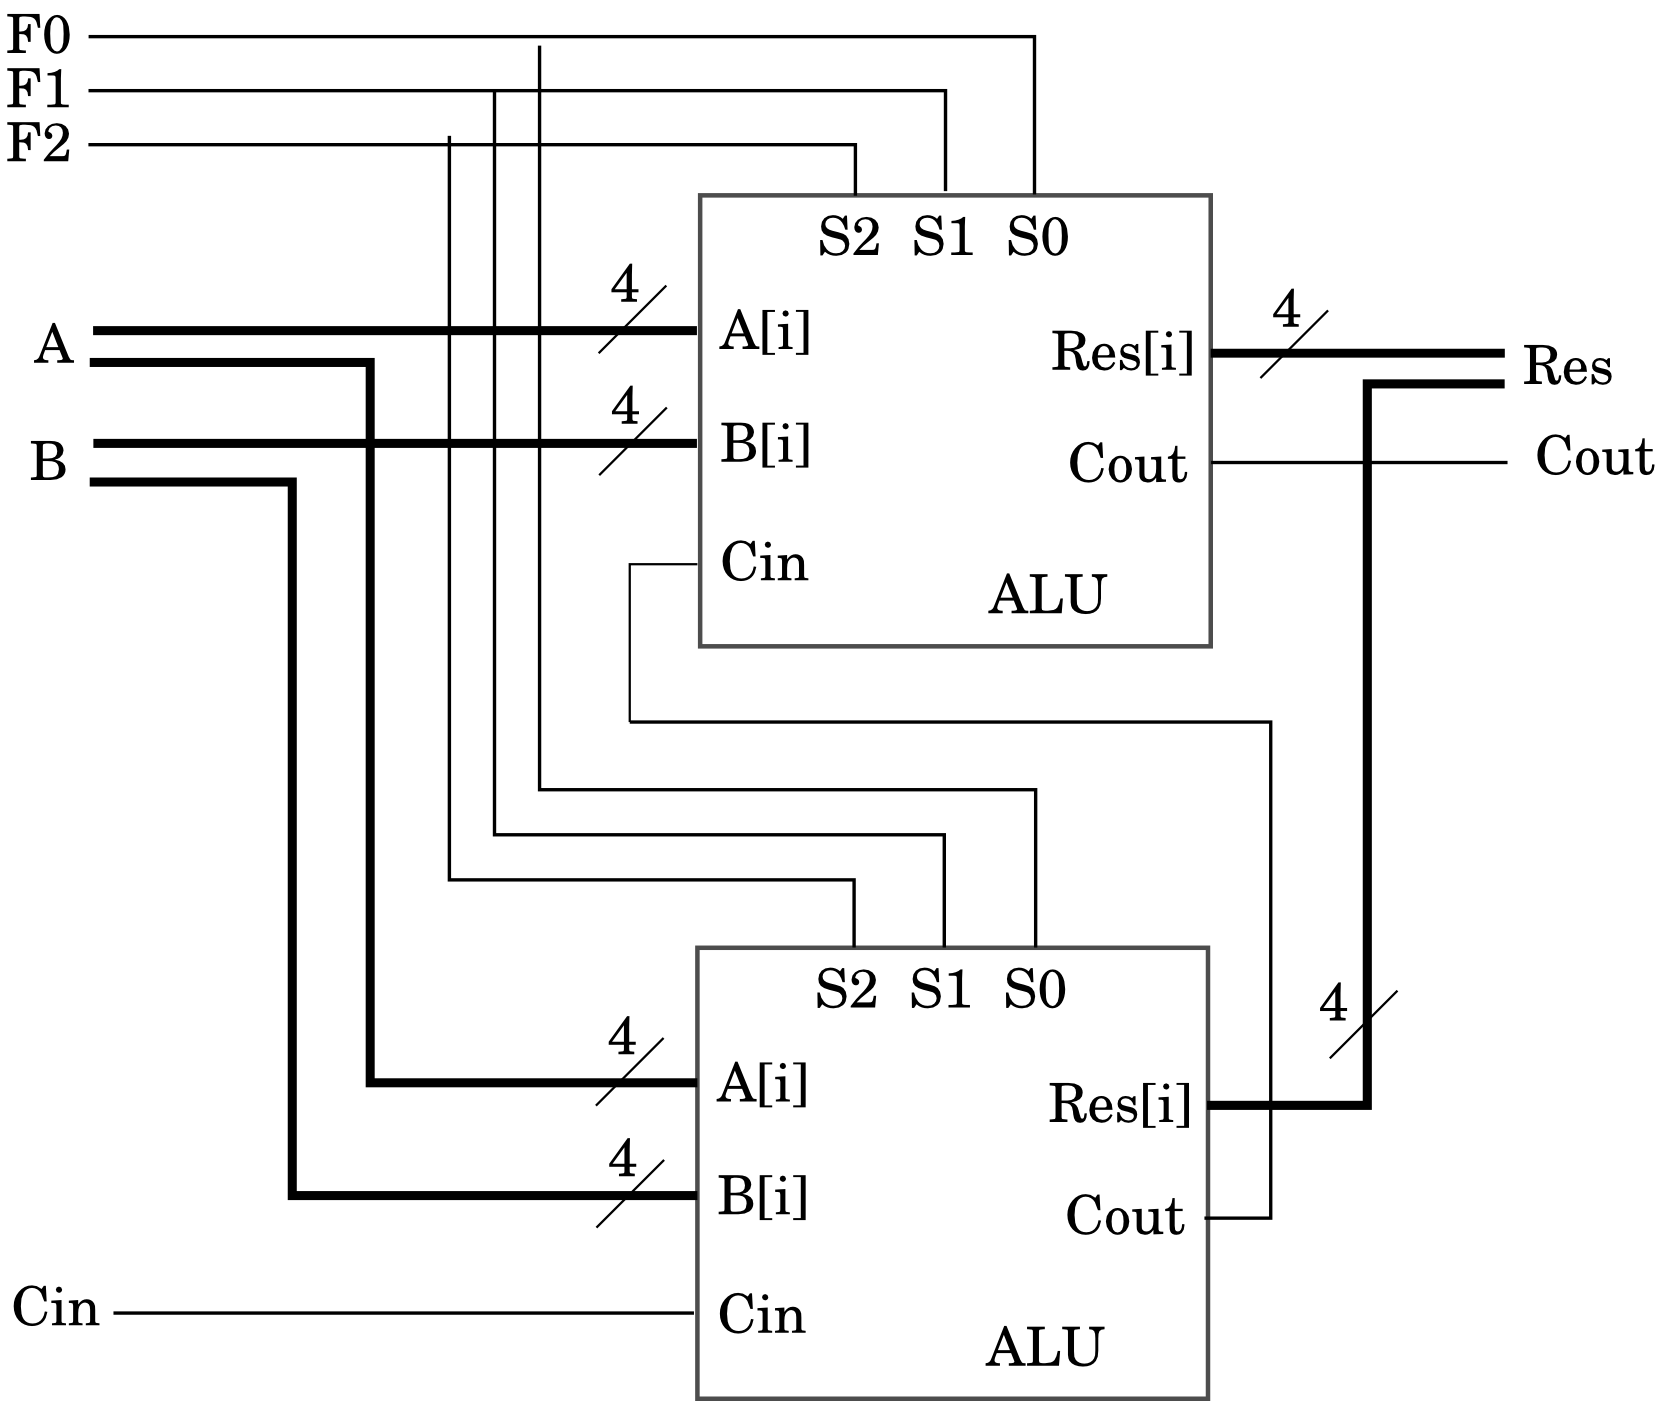
\includegraphics[width=0.2\paperwidth]{img/alu8}
\end{figure}



\paragraph{The Shifter}

We can very easily design an eight function shifter:

\begin{figure}[H]
\noindent \centering{}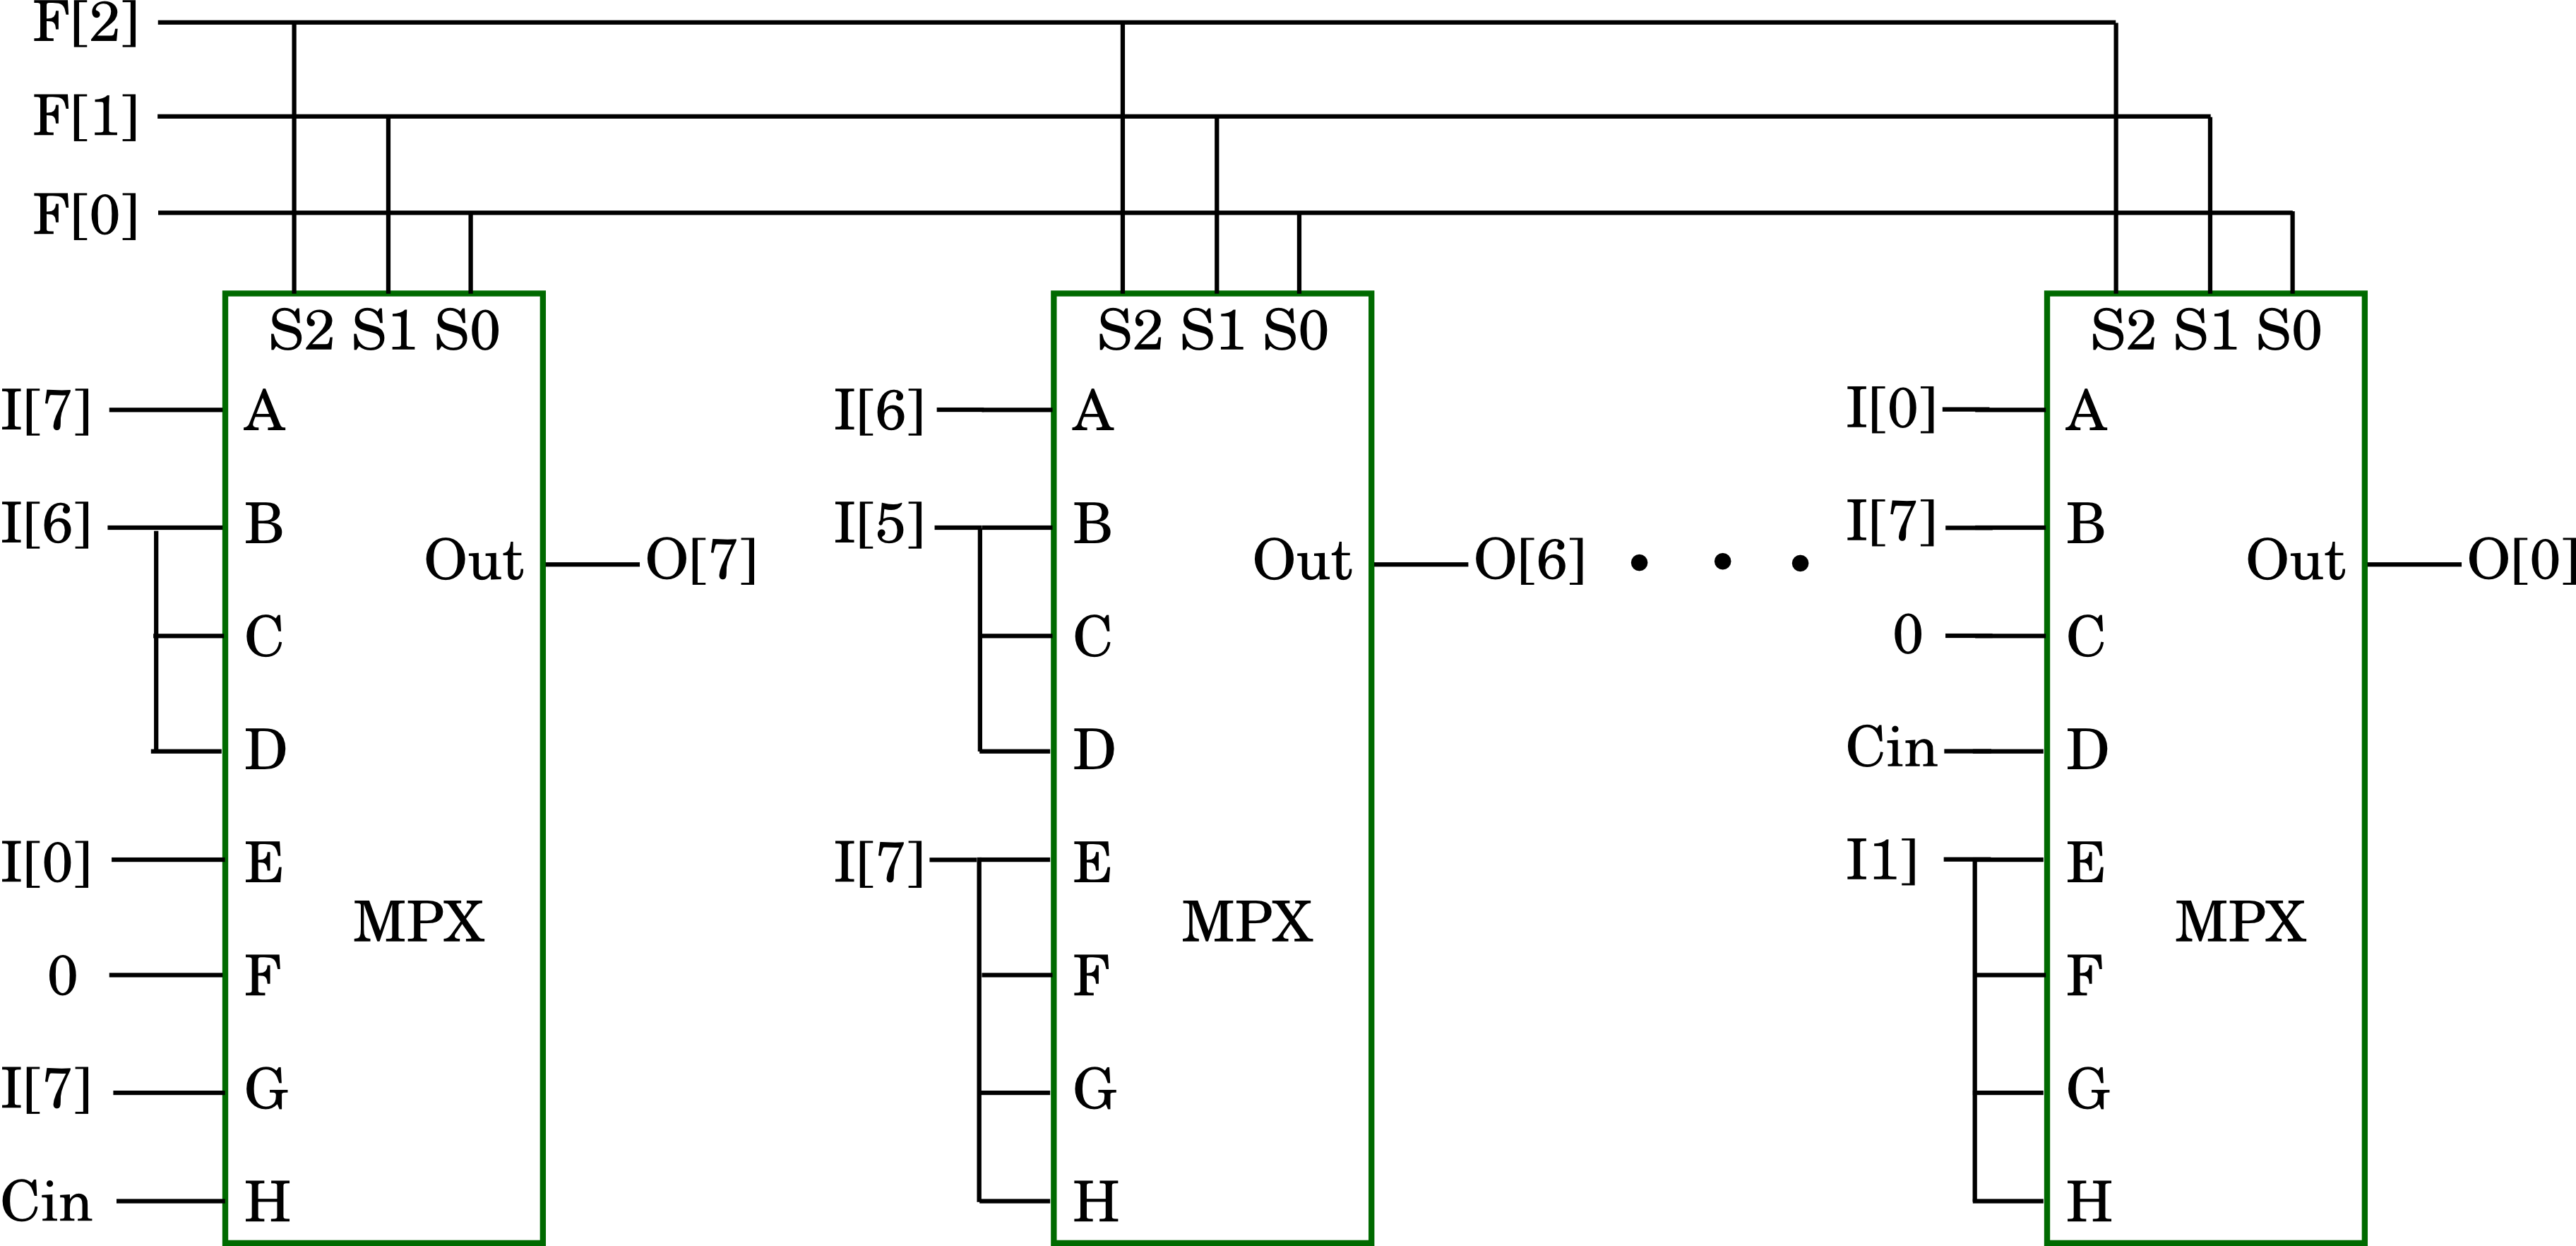
\includegraphics[width=0.3\paperwidth]{img/shifter}
\end{figure}


Here we have the functions: \textbf{A} - unchanged, \textbf{B} - rotate
left, \textbf{C} - arithmetic left shift, \textbf{D} - left shift
with carry, \textbf{E} - rotate right, \textbf{F} - logical right
shift, \textbf{G} - arithmetic right shify, \textbf{H} - right shift
with carry.


\section{Processors}

\begin{figure}[H]
\textbf{A Manual Processor Data Path Diagram}

\noindent \centering{}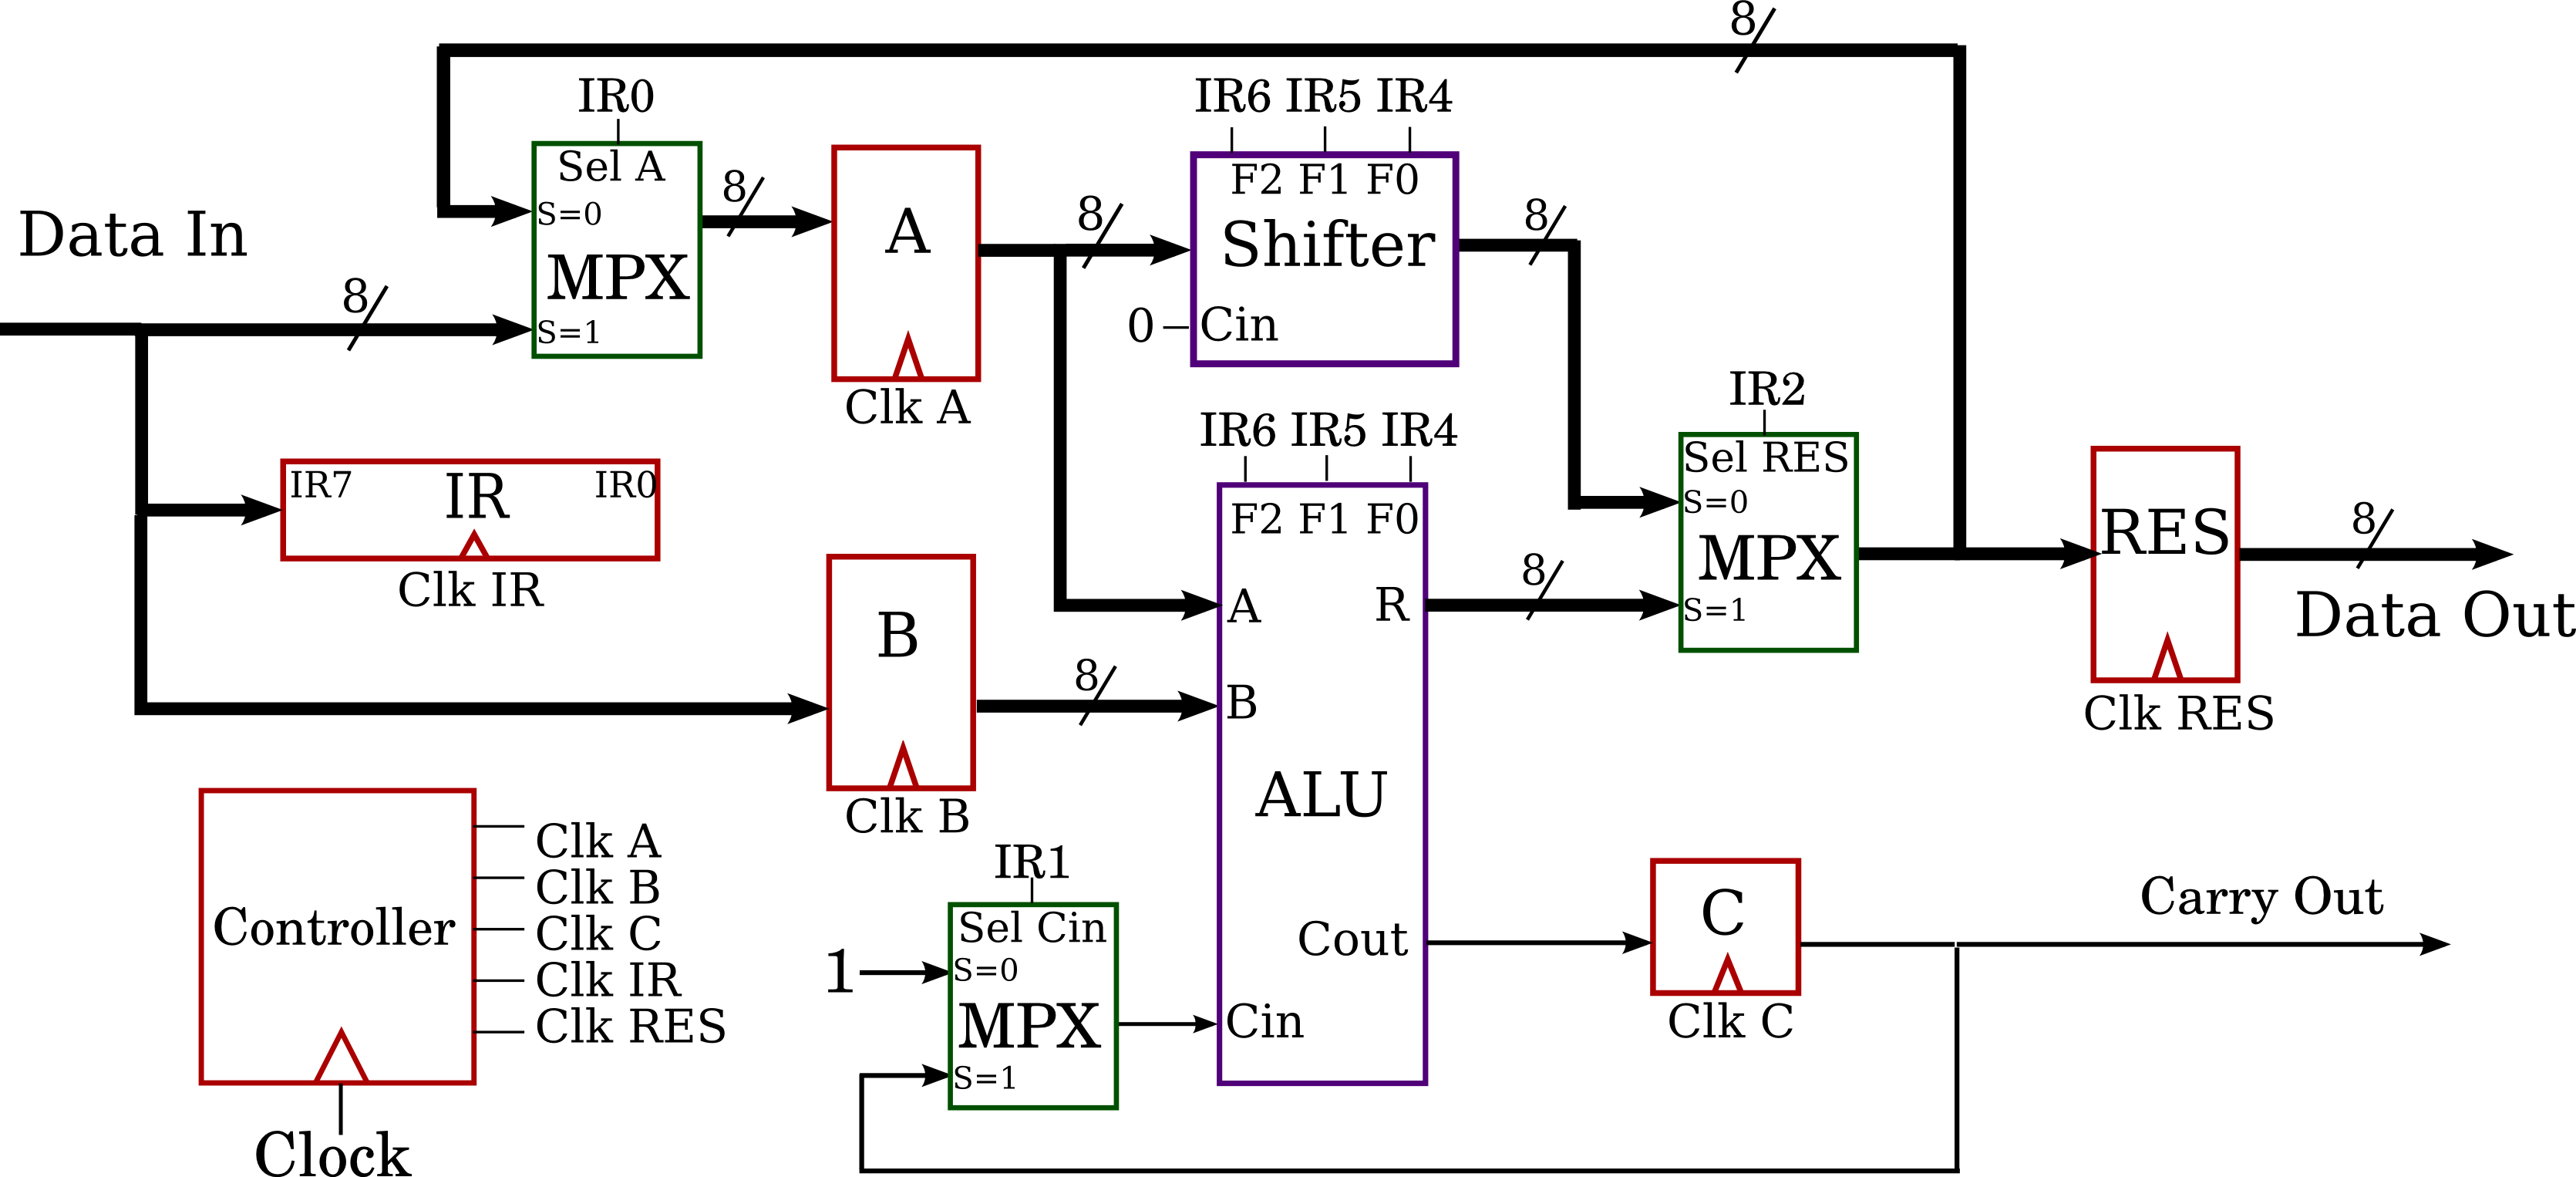
\includegraphics[width=0.325\paperwidth]{img/manualpdpd}
\end{figure}



\paragraph{\noindent Instruction Format}

\noindent We define the instruction register hold instructions as
follows:

\noindent 
\begin{table}[H]
\noindent \centering{}%
\begin{tabular}{cccccccc}
\toprule 
IR7 & IR6 & IR5 & IR4 & IR3 & IR2 & IR1 & IR0\tabularnewline
\midrule 
UN & \multicolumn{3}{c}{F/ALU-SHIFT} & UN & S/R & S/C & S/A\tabularnewline
\bottomrule
\end{tabular}
\end{table}

\begin{itemize}
\item S/A selects input to A register.
\item S/C selects input to ``Carry in'' of ALU.
\item S/R selects input to RES-register.
\item F/ALU determinse function of ALU/shifter. 000 for \textbf{A}, ...,
111 for \textbf{H}.
\item Bits 3 and 7 are unused.
\end{itemize}

\paragraph{Execution Cycle}
\begin{enumerate}
\item Load IR register.
\item Load A register.
\item Load B, C registers.
\item Load IR register.
\item Load RES, C registers.
\end{enumerate}

\paragraph{Example Sequential Circuit Design}

For a manual processor:

\emph{1. State Assignment}

\noindent 
\begin{table}[H]
\noindent \begin{centering}
{\footnotesize{}Chosen to minimise output logic:}
\par\end{centering}{\footnotesize \par}

\smallskip{}


\noindent \centering{}%
\begin{tabular}{ccc}
\toprule 
{\footnotesize{}$Q_{2}Q_{1}Q_{0}$} & {\footnotesize{}State} & {\footnotesize{}Output}\tabularnewline
\midrule 
{\footnotesize{}000} & {\footnotesize{}0} & {\footnotesize{}none}\tabularnewline
{\footnotesize{}001} & {\footnotesize{}1} & {\footnotesize{}ClkIR}\tabularnewline
{\footnotesize{}100} & {\footnotesize{}2} & {\footnotesize{}ClkA}\tabularnewline
{\footnotesize{}010} & {\footnotesize{}3} & {\footnotesize{}ClkB, ClkC}\tabularnewline
{\footnotesize{}101} & {\footnotesize{}4} & {\footnotesize{}ClkIR}\tabularnewline
{\footnotesize{}110} & {\footnotesize{}5} & {\footnotesize{}ClkC, ClkRES}\tabularnewline
\bottomrule
\end{tabular}
\end{table}


\emph{2. State Transition Diagram}

\begin{figure}[H]
\noindent \centering{}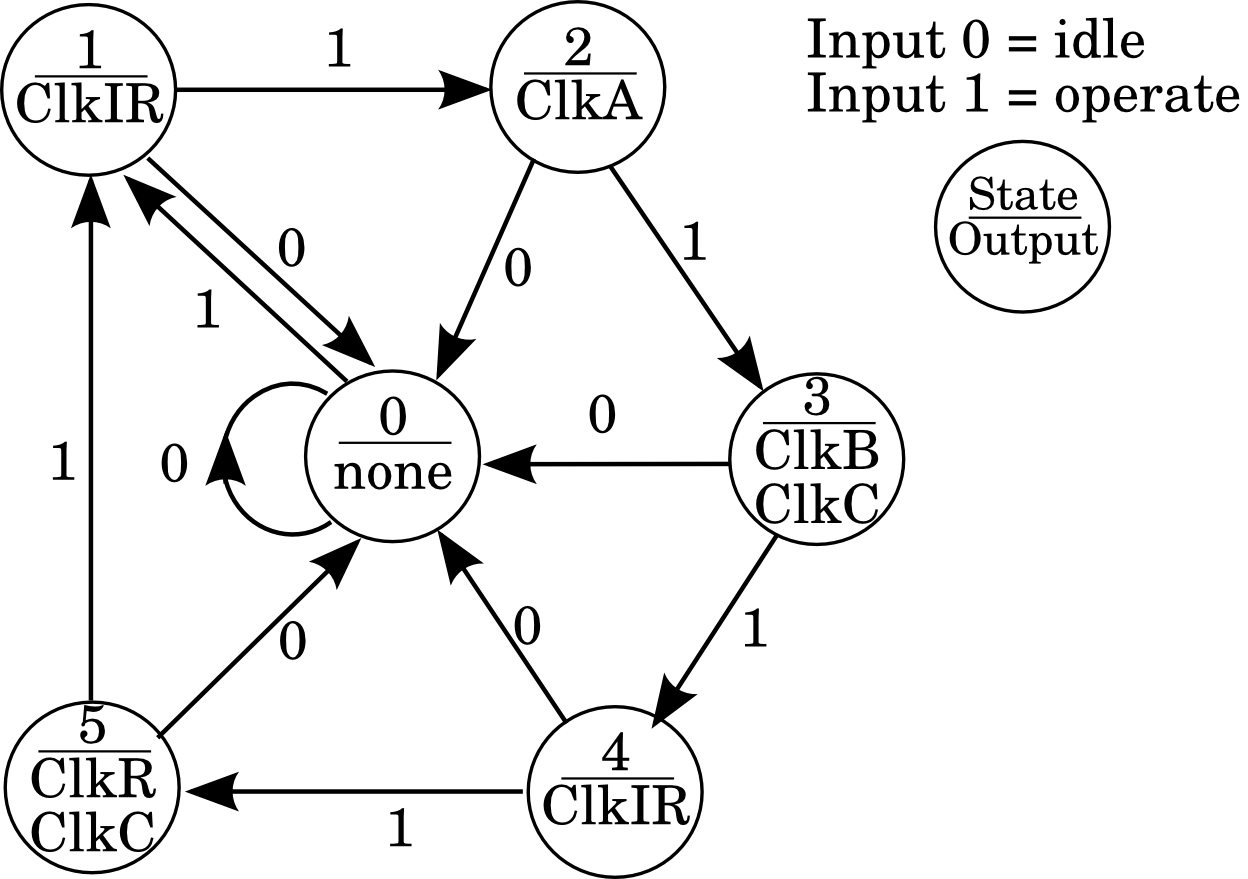
\includegraphics[width=0.15\paperwidth]{img/excycle}
\end{figure}


\emph{2. State Transition Table}

\noindent 
\begin{table}[H]
\noindent \centering{}%
\begin{tabular}{ccccccc}
\toprule 
{\footnotesize{}Operate} & {\footnotesize{}This State} & {\footnotesize{}$Q_{2}Q_{1}Q_{0}$} & {\footnotesize{}Next State} & {\footnotesize{}$D_{2}$} & {\footnotesize{}$D_{1}$} & {\footnotesize{}$D_{0}$}\tabularnewline
\midrule 
{\footnotesize{}0} & {\footnotesize{}0} & {\footnotesize{}000} & {\footnotesize{}0} & {\footnotesize{}0} & {\footnotesize{}0} & {\footnotesize{}0}\tabularnewline
{\footnotesize{}0} & {\footnotesize{}1} & {\footnotesize{}001} & {\footnotesize{}0} & {\footnotesize{}0} & {\footnotesize{}0} & {\footnotesize{}0}\tabularnewline
{\footnotesize{}0} & {\footnotesize{}2} & {\footnotesize{}100} & {\footnotesize{}0} & {\footnotesize{}0} & {\footnotesize{}0} & {\footnotesize{}0}\tabularnewline
{\footnotesize{}0} & {\footnotesize{}3} & {\footnotesize{}010} & {\footnotesize{}0} & {\footnotesize{}0} & {\footnotesize{}0} & {\footnotesize{}0}\tabularnewline
{\footnotesize{}0} & {\footnotesize{}4} & {\footnotesize{}101} & {\footnotesize{}0} & {\footnotesize{}0} & {\footnotesize{}0} & {\footnotesize{}0}\tabularnewline
{\footnotesize{}0} & {\footnotesize{}5} & {\footnotesize{}110} & {\footnotesize{}0} & {\footnotesize{}0} & {\footnotesize{}0} & {\footnotesize{}0}\tabularnewline
{\footnotesize{}0} & {\footnotesize{}6} & {\footnotesize{}011} & {\footnotesize{}$\times$} & {\footnotesize{}$\times$} & {\footnotesize{}$\times$} & {\footnotesize{}$\times$}\tabularnewline
{\footnotesize{}0} & {\footnotesize{}7} & {\footnotesize{}111} & {\footnotesize{}$\times$} & {\footnotesize{}$\times$} & {\footnotesize{}$\times$} & {\footnotesize{}$\times$}\tabularnewline
\midrule
{\footnotesize{}1} & {\footnotesize{}0} & {\footnotesize{}000} & {\footnotesize{}1} & {\footnotesize{}0} & {\footnotesize{}0} & {\footnotesize{}1}\tabularnewline
{\footnotesize{}1} & {\footnotesize{}1} & {\footnotesize{}001} & {\footnotesize{}2} & {\footnotesize{}1} & {\footnotesize{}0} & {\footnotesize{}0}\tabularnewline
{\footnotesize{}1} & {\footnotesize{}2} & {\footnotesize{}100} & {\footnotesize{}3} & {\footnotesize{}0} & {\footnotesize{}1} & {\footnotesize{}0}\tabularnewline
{\footnotesize{}1} & {\footnotesize{}3} & {\footnotesize{}010} & {\footnotesize{}4} & {\footnotesize{}1} & {\footnotesize{}0} & {\footnotesize{}1}\tabularnewline
{\footnotesize{}1} & {\footnotesize{}4} & {\footnotesize{}101} & {\footnotesize{}5} & {\footnotesize{}1} & {\footnotesize{}1} & {\footnotesize{}0}\tabularnewline
{\footnotesize{}1} & {\footnotesize{}5} & {\footnotesize{}110} & {\footnotesize{}1} & {\footnotesize{}0} & {\footnotesize{}0} & {\footnotesize{}1}\tabularnewline
{\footnotesize{}1} & {\footnotesize{}6} & {\footnotesize{}011} & {\footnotesize{}$\times$} & {\footnotesize{}$\times$} & {\footnotesize{}$\times$} & {\footnotesize{}$\times$}\tabularnewline
{\footnotesize{}1} & {\footnotesize{}7} & {\footnotesize{}111} & {\footnotesize{}$\times$} & {\footnotesize{}$\times$} & {\footnotesize{}$\times$} & {\footnotesize{}$\times$}\tabularnewline
\bottomrule
\end{tabular}
\end{table}


\emph{3. State Sequencing Logic - Karnaugh Maps and Boolean Eqns}

\begin{figure}[H]
\noindent \centering{}\includegraphics[width=0.2\paperwidth]{img/ssl-kmaps}
\end{figure}


\emph{4. Checking Don't Cares}

\noindent 
\begin{table}[H]
\noindent \begin{centering}
\begin{tabular}{ccccccc}
\toprule 
{\footnotesize{}Operate} & {\footnotesize{}This State} & {\footnotesize{}$Q_{2}Q_{1}Q_{0}$} & {\footnotesize{}Next State} & {\footnotesize{}$D_{2}$} & {\footnotesize{}$D_{1}$} & {\footnotesize{}$D_{0}$}\tabularnewline
\midrule
{\footnotesize{}0} & {\footnotesize{}6} & {\footnotesize{}011} & {\footnotesize{}0} & {\footnotesize{}0} & {\footnotesize{}0} & {\footnotesize{}0}\tabularnewline
{\footnotesize{}0} & {\footnotesize{}7} & {\footnotesize{}111} & {\footnotesize{}0} & {\footnotesize{}0} & {\footnotesize{}0} & {\footnotesize{}0}\tabularnewline
\midrule
{\footnotesize{}1} & {\footnotesize{}6} & {\footnotesize{}011} & {\footnotesize{}4} & {\footnotesize{}1} & {\footnotesize{}0} & {\footnotesize{}1}\tabularnewline
{\footnotesize{}1} & {\footnotesize{}7} & {\footnotesize{}111} & {\footnotesize{}4} & {\footnotesize{}1} & {\footnotesize{}0} & {\footnotesize{}1}\tabularnewline
\bottomrule
\end{tabular}
\par\end{centering}

\smallskip{}


\noindent \centering{}{\footnotesize{}So if the OPERATE input is at
0 when the processor is switched on, the system will begin in IDLE
state.}{\footnotesize \par}
\end{table}


\emph{5. Output Logic - Karnaugh Maps and Boolean Eqns}

\begin{figure}[H]
\noindent \begin{centering}
\includegraphics[width=0.24\paperwidth]{img/ol-kmaps}
\par\end{centering}

\noindent \centering{}\includegraphics[width=0.16\paperwidth]{img/ol-kmaps'}
\end{figure}


\emph{{*}. Connecting Output to the System Clock}

\begin{figure}[H]
\noindent \begin{centering}
\includegraphics[width=0.175\paperwidth]{img/output-clock}
\par\end{centering}

\smallskip{}


\noindent \centering{}{\footnotesize{}We use a NAND gate to connect
each output to the system clock. This means the state register changes
on the falling edge, avoiding race conditions when the next state
is set on the following rising edge.}{\footnotesize \par}
\end{figure}


\emph{We now have a manual processor!}


\paragraph{Memory}
\begin{itemize}
\item A D-type flip flop is a one bit memory.
\item We need to give it an address (binary number). We use a demultiplexer
to do this.
\end{itemize}
\begin{figure}[H]
\noindent \centering{}\includegraphics[width=0.2\paperwidth]{img/addr-memory}
\end{figure}



\paragraph{Buses}

E.g. address bus, data buses, control bus.
\begin{itemize}
\item Data-in and data-out are never used at the same time. Convenient to
use one (bi-directonal) bus. This requires a tri-state buffer.
\end{itemize}

\paragraph{Tri-State Buffer}

If $C$ is 0, ouput follows $D$, otherwise is disconnected completely.

\begin{figure}[H]
\noindent \centering{}\includegraphics[width=0.075\paperwidth]{img/tri-state}
\end{figure}


We can use a demultiplexer to make sure only one input has $C$ set
to 0.


\paragraph{Random Access Memory}

Normally organised in two dimensions with row and column decoders.

\begin{figure}[H]
\noindent \centering{}\includegraphics[width=0.275\paperwidth]{img/ram-layout}
\end{figure}

\begin{itemize}
\item Each memory cell enabled when both row and column lines are 1.
\item Only ever one such cell. 
\item Each cell connected to same read/write line and data line.
\item Data line connected to outside through a two-way tri state buffer,
so unless the chip is enabled, no data can pass in or our. Allows
RAM with several chips.
\end{itemize}

\paragraph{Connecting RAM to a Processor}
\begin{itemize}
\item Need Memory Address Register (MAR) to store address.
\item Memory Data Register (MDR) to store data read from memory / to be
written to memory.
\item Program counter (PC) stores address of next program instruction to
be executed.
\item Instruction register (IR) stores the program instruction executed.
\end{itemize}
\begin{figure}[H]
\noindent \centering{}\includegraphics[width=0.3\paperwidth]{img/mem-proc}
\end{figure}



\paragraph{Fetch Cycle}

To retrieve data from memory we go through register transfer steps.
E.g. to get the next program instruction and load it into the IR:
\begin{enumerate}
\item $\mbox{MAR}\leftarrow\mbox{PC}$
\item $\mbox{MDR}\leftarrow\mbox{RAM}\left[\mbox{MAR}\right]$, $\mbox{PC}\rightarrow\mbox{PC}+1$
\item $\mbox{IR}\leftarrow\mbox{MDR}$
\end{enumerate}

\paragraph{Controller}
\begin{itemize}
\item Sets multiplexers to establish required connection paths.
\item Gives falling edge signal to clock inputs of registers to be loaded
(done by gating system clock - NAND with clock control logic).
\item Is a synchronous sequential circuit.
\end{itemize}

\paragraph{Dynamic RAM}

For large RAMs, D-Q flip flops are to big, instead one transistor
and capacitor is used for each bit. Value = whether capacitor is charged.
\begin{itemize}
\item Store is not permanent, ones drift to zero quickly.
\item Capacitor charge is restored regularly, done by memory controller
when the computer not accessing memory.
\end{itemize}

\paragraph{Speeding Up the Processor}
\begin{itemize}
\item Change buses from 8 to 32 bit.
\item Provide local registers which can be programmed to store partial results.
\item Design a controller with as small a number of execution cycles as
possible.
\item Remove carry arrangments, doing arithmetic on big integers.
\item Replace bi-directional data bus with seperate data in and data out
buses.
\end{itemize}
\begin{figure}[H]
\noindent \centering{}\includegraphics[width=0.325\paperwidth]{img/32-processor}
\end{figure}



\paragraph{Defining Operations}

E.g. LOAD, using register transfer language:

\noindent 
\begin{table}[H]
\noindent \centering{}%
\begin{tabular}{cccc}
\toprule 
{\footnotesize{}Instruction} & {\footnotesize{}Cycle} & {\footnotesize{}Transfers} & {\footnotesize{}Path}\tabularnewline
\midrule 
\multirow{3}{*}{{\footnotesize{}LOAD Rdst, Addr}} & {\footnotesize{}E1} & {\footnotesize{}MAR$\leftarrow$MDR} & {\footnotesize{}Via bit mask}\tabularnewline
 & {\footnotesize{}E2} & {\footnotesize{}MDR$\leftarrow$Memory} & \tabularnewline
 & {\footnotesize{}E3} & {\footnotesize{}Rdst$\leftarrow$MDR} & {\footnotesize{}No mask}\tabularnewline
\bottomrule
\end{tabular}
\end{table}


Instruction format: 8 bits for the opcode, 4 for Rdest, 20 for address.


\paragraph{Designing the Controller}
\begin{itemize}
\item Define a control input based on how many cycles required for each
operation.

\begin{itemize}
\item Using 8-to-256 decoder to decode the opcode.
\item Using 3-to-8 decoder for current state.
\end{itemize}
\item Sequential design problem to work out next state, uses this control
input and previous state.
\item Output logic:

\begin{itemize}
\item Clocks: NAND gates with system clock. In practice, we can simplify
output logic by considering the following cycle.
\item Multiplexers and ALU / Shifter function selection output is trivial.
\end{itemize}
\end{itemize}

\paragraph{Possible Improvements}
\begin{itemize}
\item Instructions packed on byte boundaries so not to waste fetch cycles.
\item Additional arithmetic hardware.
\item Additional multiplexers, e.g. to select input of B independently of
A.\end{itemize}

\end{document}
